\subsection{Generating Modules and Finitely Generated Projective Modules}

PROPOSITION 2. --- Let A and B be algebras over k, and let P be an \((A,B)_{k}\) -bimodule. Suppose that the mapping \(b \mapsto b_{P}\) from B to \(\operatorname{End}_{\mathrm{A}}(\mathrm{P})\) is bijective. The following assertions are equivalent:

\begin{enumerate}
\def\labelenumi{(\roman{enumi})}
\item
  The A-module P is projective and finitely generated.
\item
  The mapping \(\Theta\) (VIII, p.~96) is an isomorphism of \((\mathrm{B},\mathrm{B})_k\) -bimodules from \(\mathrm{P}^* \otimes_{\mathrm{A}} \mathrm{P}\) to \(s\mathrm{B}_d\) .
\item
  The image of \(\Theta\) contains the unit element of B.
\end{enumerate}

If, moreover, the mapping \(a \mapsto a_{P}\) from A to \(\operatorname{End}_{\mathrm{B}}(\mathrm{P})\) is bijective, then the assertions above are equivalent to the following statement:

\begin{enumerate}
\def\labelenumi{(\roman{enumi})}
\setcounter{enumi}{3}
\tightlist
\item
  There exist a \((\mathrm{B},\mathrm{A})_{k}\) -bimodule Q and a surjective homomorphism of \((\mathrm{B},\mathrm{B})_{k}\) -bimodules from \(Q\otimes_{A}P\) to \(_{s}B_{d}\) .
\end{enumerate}

By the corollary of II, §4, No.~2, p.~271, assertion (i) implies (ii). Moreover, (iii) follows from (ii). Let \(t \in \mathrm{B}^* \otimes_{\mathrm{A}} \mathrm{B}\) be such that \(\Theta(t) = 1\) . Let \(n\) be an integer, and let \((x_1, \ldots, x_n) \in \mathrm{P}^n\) and \((x_1^*, \ldots, x_n^*) \in \mathrm{P}^{*n}\) be such that \(t = \sum_{i=1}^{n} x_i^* \otimes x_i\) . For every \(x\) belonging to \(\mathrm{P}\) , the relation \(x\Theta(t) = x\) can be written as

\[
\sum_ {i = 1} ^ {n} \langle x, x _ {i} ^ {*} \rangle x _ {i} = x.
\]

It follows that the A-module P is finitely generated by the family \((x_{i})_{1\leqslant i\leqslant n}\) , and we conclude the proof of the implication (iii) \(\Rightarrow\) (i) using Proposition 12 of II, §2, No.~6, p.~238.

We obviously have (ii) \(\Rightarrow\) (iv). Let \(Q\) be a \((B,A)_k\) -bimodule and \(\theta\) a surjective homomorphism of \((B,B)_k\) -bimodules from \(Q \otimes_A P\) to \(s B_d\) . In the notation of the previous subsection, there exists a homomorphism of \((B,A)_k\) -bimodules \(\zeta: Q \to \widetilde{P}\) such that \(\theta(y \otimes x) = \langle \zeta(y), x \rangle\) for \(x \in P\) and \(y \in Q\) , and we have \(\theta = \widetilde{\Lambda} \circ (\zeta \otimes 1_P)\) . Since \(\theta\) is surjective, the same holds for \(\widetilde{\Lambda}\) . If the mapping \(a \mapsto a_P\) from \(A\) to \(\mathrm{End}_B(P)\) is bijective, then \(\Theta\) is surjective by relation (14) of Proposition 1 of VIII, p.~97; the implication (iv) \(\Rightarrow\) (iii) follows.

PROPOSITION 3. --- Let A and B be algebras over k and P an \((A,B)_{k}\) -bimodule. The following properties are equivalent:

\begin{enumerate}
\def\labelenumi{(\roman{enumi})}
\item
  The A-module P is generating.
\item
  The image of the mapping \(\Lambda\) from \(\mathrm{P} \otimes_{\mathrm{B}} \mathrm{P}^{*}\) to \(s\mathrm{A}_{d}\) (VIII, p.~95) contains the unit element.
\item
  There exist a \((\mathrm{B},\mathrm{A})_{k}\) -bimodule Q and a surjective homomorphism of \((\mathrm{A},\mathrm{A})_{k}\) -bimodules from \(P\otimes_{B}Q\) to \(_{s}A_{d}\) .
\end{enumerate}

If, moreover, the mapping \(b \mapsto b_{P}\) from B to \(\operatorname{End}_{\mathrm{A}}(\mathrm{P})\) is bijective, then the assertions are equivalent to the following statement:

\begin{enumerate}
\def\labelenumi{(\roman{enumi})}
\setcounter{enumi}{3}
\tightlist
\item
  The mapping \(\Lambda\) is an isomorphism from \(\mathrm{P} \otimes_{\mathrm{B}} \mathrm{P}^{*}\) to \(s\mathrm{A}_d\) .
\end{enumerate}

(i) \(\Leftrightarrow\) (ii): The image of \(\Lambda\) is the trace ideal \(\tau(\mathrm{P})\) (VIII, p.~80). The equivalence of (i) and (ii) therefore follows from Theorem 1 of VIII, p.~80.

(ii) \(\Rightarrow\) (iii): It suffices to take \(Q = P^{*}\) .

(iii) \(\Rightarrow\) (ii): Let \(Q\) be a \((B,A)_k\) -bimodule and \(\psi\) a homomorphism of \((A,A)_k\) -bimodules from \(P \otimes_B Q\) to \({}_s A_d\) . There exists a homomorphism of \((B,A)_k\) -bimodules \(\Psi\) from \(Q\) to \(P^*\) such that \(\psi(x \otimes y) = \langle x, \Psi(y) \rangle\) for \(x \in P\) and \(y \in Q\) , and we have the equality \(\psi = \Lambda \circ (1_P \otimes \Psi)\) . If \(\psi\) is surjective, then so is \(\Lambda\) .

It is clear that (iv) implies (ii). Conversely, suppose that property (ii) holds and that the mapping \(b \mapsto b_{P}\) from B to \(\operatorname{End}_{\mathrm{A}}(\mathrm{P})\) is bijective. Let e be an element of \(P \otimes_{B} P^{*}\) such that \(\Lambda(e) = 1\) . By relation (7) of VIII, p.~96, we have \(u = \Lambda(u)e\) for every u in \(P \otimes_{B} P^{*}\) ; the injectivity of \(\Lambda\) follows.

PROPOSITION 4. --- Let A and B be k-algebras and P an \((\mathrm{A},\mathrm{B})_{k}\) -bimodule. Suppose that the mapping \(b\mapsto b_{P}\) from B to \(\operatorname{End}_{\mathrm{A}}(\mathrm{P})\) is bijective.

\begin{enumerate}
\def\labelenumi{\alph{enumi})}
\item
  If the A-module P is generating, then the right B-module P is projective and finitely generated.
\item
  If the A-module P is projective and finitely generated, then the right B-module P is generating.
\end{enumerate}

Suppose that the A-module P is generating. It is then faithful and balanced (VIII, p.~82, Theorem 2), and consequently the mapping \(a \mapsto a_{\mathrm{P}}\) from A to \(\mathrm{End}_{\mathrm{B}}(\mathrm{P})\) is bijective (VIII, p.~97, Remark 1). Moreover, the mapping \(\Lambda : \mathrm{P} \otimes_{\mathrm{B}} \mathrm{P}^{*} \to {}_{s} \mathrm{A}_{d}\) is bijective (VIII, p.~98, Proposition 3). We view P as a \((\mathrm{B}^{\circ}, \mathrm{A}^{\circ})_{k}\) -bimodule. The mapping \(\Lambda\) induces a bijective mapping \(\mathrm{P}^{*} \otimes_{\mathrm{B}^{\circ}} \mathrm{P} \to \mathrm{A}^{\circ}\) ; by Proposition 2 of VIII, p.~98, (iv) \(\Rightarrow\) (i), the right B-module P is projective and finitely generated.

Now, suppose that the A-module P is projective and finitely generated. Then the mapping \(\Theta: P^{*} \otimes_{A} P \to_{s} B_{d}\) is bijective (loc. cit., (i) \(\Rightarrow\) (ii)). By the implication (iii) \(\Rightarrow\) (i) of Proposition 3 above applied to the \((\mathrm{B}^{\circ}, \mathrm{A}^{\circ})_{k}\) -bimodule P, the right B-module P is generating.

COROLLARY 1. --- The countermodule of a generating module is projective and finitely generated. The countermodule of a finitely generated projective module is generating.

Let A be a k-algebra, and let M be an A-module. We denote the opposite k-algebra of the algebra \(\operatorname{End}_{\mathrm{A}}(\mathrm{M})\) by B. The corollary follows from Proposition 4 applied to the \((\mathrm{A},\mathrm{B})_{k}\) -bimodule M.

COROLLARY 2. --- Let A and B be k-algebras and P an \((A,B)_{k}\) -bimodule. The following properties are equivalent:

\begin{enumerate}
\def\labelenumi{(\roman{enumi})}
\item
  The A-module P is generating, and the mapping \(b \mapsto b_{P}\) from B to \(\operatorname{End}_{\mathrm{A}}(\mathrm{P})\) is bijective.
\item
  The right B-module P is projective, finitely generated, faithful, and balanced, and the mapping \(a \mapsto a_{\mathrm{P}}\) from A to \(\operatorname{End}_{\mathrm{B}}(\mathrm{P})\) is bijective.
\end{enumerate}

The implication \((i) \Rightarrow (ii)\) follows from Proposition 4, a) and Remark 1 (VIII, p.~97). Assume that (ii) holds; then the A-module P is generating (Proposition 4, b) applied to the \((B^{\circ}, A^{\circ})_{k}\) -bimodule P). Since the B-module P is faithful and balanced, the second assertion of (i) is also satisfied (VIII, p.~97, Remark 1).

\subsection{Invertible Bimodules and Morita Equivalence}

DEFINITION 1. --- Let A and B be k-algebras and P an \((\mathrm{A},\mathrm{B})_{k}\) -bimodule. We say that P is invertible if there exists a \((\mathrm{B},\mathrm{A})_{k}\) -bimodule Q such that \(P \otimes_{B} Q\) is isomorphic to \(_{s}A_{d}\) and \(Q \otimes_{A} P\) to \(_{s}B_{d}\) . Such a bimodule Q is called an inverse of P.

Let A and B be k-algebras, and let P be an invertible \((\mathrm{A},\mathrm{B})_{k}\) -bimodule. Let C be a k-algebra and \(P'\) an invertible \((\mathrm{B},\mathrm{C})_{k}\) -bimodule. Finally, let Q and \(Q'\) be inverse bimodules of P and \(P'\) , respectively. By the associativity of the tensor product (II, §3, No.~8, p.~258, Proposition 8) and Proposition 4 of II, §3, No.~4, p.~249, the \((\mathrm{C},\mathrm{A})_{k}\) -bimodule \(Q'\otimes_{B}Q\) is an inverse of the \((\mathrm{A},\mathrm{C})_{k}\) -bimodule \(P\otimes_{B}P'\) , so that \(P\otimes_{B}P'\) is an invertible \((\mathrm{A},\mathrm{C})_{k}\) -bimodule. Hence, the relation

``A and B are k-algebras, and there exists an invertible \((A,B)_{k}\) -bimodule'' is an equivalence relation.

DEFINITION 2. --- Two k-algebras A and B are called Morita equivalent if there exists an invertible \((\mathrm{A},\mathrm{B})_{k}\) -bimodule. Rings A and B are called Morita equivalent if the Z-algebras A and B are Morita equivalent.

Two isomorphic k-algebras are Morita equivalent. If two k-algebras are Morita equivalent, then their opposite algebras are Morita equivalent.

Let P be an invertible \((\mathrm{A},\mathrm{B})_{k}\) -bimodule and Q an inverse of P. Then Q is an invertible \((\mathrm{B},\mathrm{A})_{k}\) -bimodule, and it has P as inverse. Moreover, viewed as a \((\mathrm{B}^{\circ},\mathrm{A}^{\circ})_{k}\) -bimodule, P is invertible and has the \((\mathrm{A}^{\circ},\mathrm{B}^{\circ})_{k}\) -bimodule Q as inverse.

Lemma 1. --- Let A and B be k-algebras, P be an invertible \((\mathrm{A},\mathrm{B})_{k}\) -bimodule, M and N be B-modules, and \(u:M\to N\) be a B-linear mapping. If the mapping \(1_{P}\otimes u:P\otimes_{B}M\to P\otimes_{B}N\) is zero (resp. bijective), then so is u.

Let Q be a bimodule inverse to P and \(\theta: Q \otimes_{A} P \to_{s} B_{d}\) an isomorphism of \((B, B)_{k}\) -bimodules. The lemma follows from the commutativity of the diagram

\pandocbounded{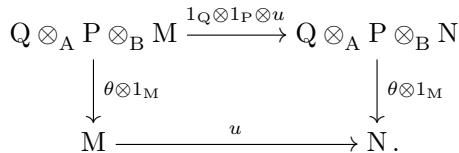
\includegraphics[keepaspectratio]{images/part001_2598f5b2.jpg}}

THEOREM 1. --- Let A and B be k-algebras and P an \((A,B)_{k}\) -bimodule. Denote the \((B,A)_{k}\) -bimodule \(\operatorname{Hom}_{\mathrm{A}}(\mathrm{P},\mathrm{A}_{s})\) by \(P^{*}\) . The following properties are equivalent:

\begin{enumerate}
\def\labelenumi{(\roman{enumi})}
\item
  The \((\mathrm{A},\mathrm{B})_k\) -bimodule P is invertible.
\item
  The A-module P is projective, finitely generated, and generating, and the mapping \(b \mapsto b_{P}\) from B to \(\operatorname{End}_{\mathrm{A}}(\mathrm{P})^{\circ}\) is a k-algebra isomorphism.
\item
  The right B-module P is projective, finitely generated, and generating, and the mapping \(a \mapsto a_{P}\) from A to \(\operatorname{End}_{\mathrm{B}}(\mathrm{P})\) is a k-algebra isomorphism. If these properties hold, then the homomorphisms
\end{enumerate}

\[
\Theta : \mathrm{P} ^ {*} \otimes \mathrm{P} \to {} _ {s} \mathrm{B} _ {d} \quad \text{and} \quad \Lambda : \mathrm{P} \otimes \mathrm{P} ^ {*} \to {} _ {s} \mathrm{A} _ {d}
\]

are isomorphisms, so that the \((\mathrm{B},\mathrm{A})_k\) -bimodule \(\mathrm{P}^*\) is an inverse of \(\mathrm{P}\) .

If property (ii) holds, then P is an invertible \((\mathrm{A},\mathrm{B})_{k}\) -bimodule with inverse \(P^{*}\) (VIII, p.~98, Proposition 2 and p.~98, Proposition 3). This proves that (ii) implies (i) and the last assertion.

Suppose that the \((\mathrm{A},\mathrm{B})_{k}\) -bimodule P is invertible. Then the A-module P is generating (VIII, p.~98, Proposition 3, (iii) \(\Rightarrow\) (i)). It is therefore faithful and balanced (VIII, p.~82, Theorem 2) and, consequently, the mapping \(a \mapsto a_{p}\) from A to \(\operatorname{End}_{\mathrm{B}}(\mathrm{P})\) is bijective.

Let us now prove that the mapping \(b \mapsto b_{\mathrm{P}}\) from B to \(\mathrm{End}_{\mathrm{A}}(\mathrm{P})\) is bijective. Let Q be a \((\mathrm{B},\mathrm{A})_k\) -bimodule, inverse to P. Let \(u \in \mathrm{End}_{\mathrm{A}}(\mathrm{P})\) ; then \(1_{\mathrm{Q}} \otimes u\) is an endomorphism of the left B-module \(\mathbf{Q} \otimes_{\mathrm{A}} \mathbf{P}\) . Since the \((\mathrm{B},\mathrm{B})_k\) -bimodule \(\mathbf{Q} \otimes_{\mathrm{A}} \mathbf{P}\) is isomorphic to \({}_s\mathbf{B}_d\) , there exists a unique element \(b\) of B such that \(1_{\mathrm{Q}} \otimes u\) is the homothety with ratio \(b\) of the right B-module \(\mathbf{Q} \otimes_{\mathrm{A}} \mathbf{P}\) . Consequently, we have \(1_{\mathrm{Q}} \otimes (u - b_{\mathrm{P}}) = 0\) . Hence, \(u = b_{\mathrm{P}}\) by Lemma 1; this proves that the mapping \(b \mapsto b_{\mathrm{P}}\) from B to \(\operatorname{End}_{\mathrm{A}}(\mathrm{P})\) is bijective.

By Proposition 2 of VIII, p.~98, the A-module P is then projective and finitely generated. We have therefore proved the equivalence of (i) and (ii).

By interchanging the roles of A and B, we obtain the equivalence of (i) and (iii), which concludes the proof of the proposition.

COROLLARY 1. --- Let A and B be Morita equivalent k-algebras, and let P be an invertible \((A,B)_{k}\) -bimodule. There exists an isomorphism \(\varphi\) from the center \(Z(A)\) of A to the center of B determined by the relation \(\varphi(z)_{\mathrm{P}} = z_{\mathrm{P}}\) for every \(z \in Z(A)\) . The automorphisms of the \((A,B)_{k}\) -bimodule P are the homotheties \(z_{P}\) where z is an invertible element of \(Z(A)\) .

Given Theorem 1, this follows from Remark 2 of VIII, p.~97.

COROLLARY 2. --- Let A and B be Morita equivalent k-algebras, and let P be an invertible \((\mathrm{A},\mathrm{B})_{k}\) -bimodule. Every \((\mathrm{B},\mathrm{A})_{k}\) -bimodule inverse to P is isomorphic to the dual \(\mathrm{P}^{*}=\mathrm{Hom}_{\mathrm{A}}(\mathrm{P},\mathrm{A})\) of P. More precisely, let Q be a \((\mathrm{B},\mathrm{A})_{k}\) -bimodule that is an inverse of P, and let \(\lambda:P\otimes_{B}Q\to_{s}A_{d}\) be an isomorphism of \((\mathrm{A},\mathrm{A})_{k}\) -bimodules. There exists a unique mapping \(\tau:\mathrm{Q}\to\mathrm{P}^{*}\) determined by the relation \(\langle p,\tau(q)\rangle=\lambda(p\otimes q)\) for \(p\in P\) and \(q\in Q\) , and \(\tau\) is an isomorphism of \((\mathrm{B},\mathrm{A})_{k}\) -bimodules.

The existence and uniqueness of the mapping \(\tau\) are clear. It is a homomorphism of \((\mathrm{B},\mathrm{A})_{k}\) -bimodules, and we have \(\lambda=\Lambda\circ(1_{\mathrm{P}}\otimes\tau)\) . Since \(\lambda\) and \(\Lambda\) are isomorphisms of \((\mathrm{A},\mathrm{A})_{k}\) -bimodules (VIII, p.~101, Theorem 1), so is \(1_{P}\otimes\tau\) . By Lemma 1, the mapping \(\tau\) is bijective.

Remark. --- Under the assumptions of the corollary, let q be an element of Q such that we have \(\lambda(p \otimes q) = 0\) for every \(p \in P\) . We then have \(\tau(q) = 0\) , that is, q = 0. Likewise, if p is an element of P such that we have \(\lambda(p \otimes q) = 0\) for every \(q \in Q\) , then p = 0.

Examples. --- 1) Let B be a \(k\) -algebra, \(n\) an integer \(\geqslant 1\) , and A the \(k\) -algebra \(\mathbf{M}_n(\mathrm{B})\) . The right B-module \(\mathrm{P} = \mathrm{B}_d^n\) is projective, finitely generated, and generating, and A can be identified with the endomorphism algebra of P (II, §10, No.~7, p.~349). By Theorem 1, the \((\mathrm{A},\mathrm{B})_k\) -bimodule P is invertible. The algebras B and \(\mathbf{M}_n(\mathrm{B})\) are therefore Morita equivalent.

\begin{enumerate}
\def\labelenumi{\arabic{enumi})}
\setcounter{enumi}{1}
\tightlist
\item
  *Let A be a commutative \(k\) -algebra and P an A-module. We view P as an \((A, A)_k\) -bimodule whose two laws of action are equal. If the \((A, A)_k\) -bimodule P is invertible, then the A-module P is finitely generated (Theorem 1). By Theorem 3 of Comm. Alg., II, §5, No.~4, p.~114, the following properties are equivalent:
\end{enumerate}

\begin{enumerate}
\def\labelenumi{(\roman{enumi})}
\item
  The \((\mathrm{A},\mathrm{A})_{k}\) -bimodule P is invertible.
\item
  There exists an A-module \(\mathrm{Q}\) such that \(\mathrm{P} \otimes_{\mathrm{A}} \mathrm{Q}\) is isomorphic to \(\mathrm{A}\) .
\item
  The A-module P is projective, finitely generated, and of rank 1. *
\end{enumerate}

\subsection{The Morita Correspondence of Modules}

In this subsection, the letters A and B denote Morita equivalent k-algebras and P an invertible \((A,B)_{k}\) -bimodule. Choose a \((B,A)_{k}\) -bimodule Q inverse to P and isomorphisms

\[
\lambda : \mathrm{P} \otimes_ {\mathrm{B}} \mathrm{Q} \rightarrow {} _ {s} \mathrm{A} _ {d} \quad \text { and } \quad \theta : \mathrm{Q} \otimes_ {\mathrm{A}} \mathrm{P} \rightarrow {} _ {s} \mathrm{B} _ {d}.
\]

For any left B-module V, denote by \(\theta_{V}\) the homomorphism of B-modules \(\theta\otimes1_{V}:Q\otimes_{A}P\otimes_{B}V\to V\) ; it is an isomorphism since \(\theta\) is an isomorphism. Likewise, for every left A-module M, denote by \(\lambda_{M}\) the homomorphism of A-modules \(\lambda\otimes1_{M}:P\otimes_{B}Q\otimes_{A}M\to M\) ; it is an isomorphism since \(\lambda\) is an isomorphism.

THEOREM 2 (Morita). --- a) Let V and W be left B-modules. The mapping \(g \mapsto 1_{\mathrm{P}} \otimes g\) is a bijection from \(\operatorname{Hom}_{\mathrm{B}}(\mathrm{V}, \mathrm{W})\) to \(\operatorname{Hom}_{\mathrm{A}}(\mathrm{P} \otimes_{\mathrm{B}} \mathrm{V}, \mathrm{P} \otimes_{\mathrm{B}} \mathrm{W})\) . The inverse bijection sends an element h of \(\operatorname{Hom}_{\mathrm{A}}(\mathrm{P} \otimes_{\mathrm{B}} \mathrm{V}, \mathrm{P} \otimes_{\mathrm{B}} \mathrm{W})\) to the element \(\theta_{\mathrm{W}} \circ (1_{\mathrm{Q}} \otimes h) \circ \theta_{\mathrm{V}}^{-1}\) of \(\operatorname{Hom}_{\mathrm{B}}(\mathrm{V}, \mathrm{W})\) .

\begin{enumerate}
\def\labelenumi{\alph{enumi})}
\setcounter{enumi}{1}
\tightlist
\item
  Every left A-module M is isomorphic to a module of the form \(\mathrm{P} \otimes_{\mathrm{B}} \mathrm{V}\) , where V is a left B-module.
\end{enumerate}

Let V and W be left B-modules. By Lemma 1 of VIII, p.~101, the mapping \(\varphi : g \mapsto 1_{\mathrm{P}} \otimes g\) from \(\mathrm{Hom}_{\mathrm{B}}(\mathrm{V}, \mathrm{W})\) to \(\mathrm{Hom}_{\mathrm{A}}(\mathrm{P} \otimes_{\mathrm{B}} \mathrm{V}, \mathrm{P} \otimes_{\mathrm{B}} \mathrm{W})\) is injective. By interchanging the roles of P and Q (and of A and B), we see that the mapping \(\psi : h \mapsto 1_{\mathrm{Q}} \otimes h\) from \(\mathrm{Hom}_{\mathrm{A}}(\mathrm{P} \otimes_{\mathrm{B}} \mathrm{V}, \mathrm{P} \otimes_{\mathrm{B}} \mathrm{W})\) to \(\mathrm{Hom}_{\mathrm{A}}(\mathrm{Q} \otimes_{\mathrm{A}} \mathrm{P} \otimes_{\mathrm{B}} \mathrm{V}, \mathrm{Q} \otimes_{\mathrm{A}} \mathrm{P} \otimes_{\mathrm{B}} \mathrm{W})\) is also injective. Now, the composition \(\psi \circ \varphi\) is the mapping \(g \mapsto \theta_{\mathrm{W}}^{-1} \circ g \circ \theta_{\mathrm{V}}\) . It is bijective, hence so is \(\psi\) . Consequently, \(\varphi\) is bijective, and its inverse is the mapping \(h \mapsto \theta_{\mathrm{W}} \circ (1_{\mathrm{Q}} \otimes h) \circ \theta_{\mathrm{V}}^{-1}\) .

Assertion b) follows from the fact that \(\lambda_{\mathrm{M}}\) is an isomorphism from \(\mathrm{P} \otimes_{\mathrm{B}} \otimes_{\mathrm{A}} \otimes_{\mathrm{M}}\) to \(\mathrm{M}\) .

Let V be a left B-module and W a submodule of V. Since the B-module P is projective (VIII, p.~101, Theorem 1), the canonical mapping from \(P \otimes_{B} W\) to \(P \otimes_{B} V\) is injective. We identify \(P \otimes_{B} W\) with its image in \(P \otimes_{B} V\) through this mapping. We adopt the analogous conventions when P and B are replaced by Q and A.

PROPOSITION 5. --- Let V be a left B-module. The mapping \(W \mapsto P \otimes_{B} W\) is an isomorphism from the set of B-submodules of V, ordered by inclusion, to the set of A-submodules of \(P \otimes_{B} V\) , ordered by inclusion. The inverse isomorphism sends an A-submodule N of \(P \otimes_{B} V\) to the image under \(\theta_{V}\) of the B-submodule \(Q \otimes_{A} N\) of \(Q \otimes_{A} P \otimes_{B} V\) .

Denote by \(D_{\mathrm{B}}(\mathrm{V})\) the set of B-submodules of V, ordered by inclusion, and define the sets \(D_{\mathrm{A}}(\mathrm{P}\otimes_{\mathrm{B}}\mathrm{V})\) and \(D_{\mathrm{B}}(\mathrm{Q}\otimes_{\mathrm{A}}\mathrm{P}\otimes_{\mathrm{B}}\mathrm{V})\) likewise. Let \(\varphi:D_{\mathrm{B}}(\mathrm{V})\to D_{\mathrm{A}}(\mathrm{P}\otimes_{\mathrm{B}}\mathrm{V})\) be the mapping \(W\mapsto P\otimes_{B}W\) and \(\psi\) the mapping from \(D_{\mathrm{A}}(\mathrm{P}\otimes_{\mathrm{B}}\mathrm{V})\) to \(D_{\mathrm{B}}(\mathrm{Q}\otimes_{\mathrm{A}}\mathrm{P}\otimes_{\mathrm{B}}\mathrm{V})\) given by \(N\mapsto Q\otimes_{A}N\) . These are increasing mappings, and the composition \(\psi\circ\varphi\) is the mapping \(W\mapsto\theta_{\mathrm{V}}^{-1}(\mathrm{W})\) , which is bijective. Consequently, \(\varphi\) is injective, and \(\psi\) is surjective. By replacing B with A and V with \(P\otimes_{B}V\) , we see that \(\psi\) is also injective. Hence, \(\varphi\) and \(\psi\) are bijective, and the inverse mapping of \(\varphi\) is indeed that described in the proposition.

Examples. --- 1) Let us apply Proposition 5 of VIII, p.~104, to the specific case \(\mathrm{V} = \mathrm{B}_s\) .

\begin{enumerate}
\def\labelenumi{\alph{enumi})}
\item
  The mapping \(J \mapsto PJ\) is an isomorphism from the ordered set \(\mathrm{D}(\mathrm{B}_{s})\) of left ideals of B to the ordered set \(\mathrm{D}(\mathrm{P})\) of A-submodules of P. The inverse mapping sends an A-submodule M of P to the left ideal \(\mathrm{J}(\mathrm{M})\) of B consisting of the elements b of B such that M contains Pb.
\item
  The mapping \(K \mapsto KP\) is an isomorphism from the ordered set \(\mathrm{D}(A_{d})\) of right ideals of A to the ordered set \(\mathrm{D}(P)\) of B-submodules of P. The inverse mapping sends a B-submodule V of P to the right ideal \(\mathrm{K}(V)\) of A consisting of the elements a of A such that V contains aP.
\end{enumerate}

Indeed, the A-module \(P \otimes_{B} B_{s}\) can be canonically identified with P. If J is a left ideal of B, then the canonical image of \(P \otimes_{B} J\) in \(P \otimes_{B} B_{s}\) corresponds to PJ through this identification. Consequently, the mapping \(J \mapsto PJ\) is an isomorphism of ordered sets from \(D(B_{s})\) to \(D(P)\) . Let \(J \in D(B_{s})\) . Denote the set of elements b of B such that PJ contains Pb by \(J'\) . It is a left ideal of B that contains J, and we have \(PJ' \subset PJ\) . Since the mapping \(J \mapsto PJ\) is an isomorphism of ordered sets, we necessarily have \(PJ' = PJ\) and \(J = J'\) . This proves a).

Assertion b) follows from assertion a) applied to the invertible \((\mathrm{B}^{\circ},\mathrm{A}^{\circ})_{k}\) -bimodule P.

Note that the ring A is a field if and only if the B-module P is simple.

\begin{enumerate}
\def\labelenumi{\arabic{enumi})}
\setcounter{enumi}{1}
\tightlist
\item
  Denote by \(\mathcal{B}_{\mathrm{A}}\) , \(\mathcal{B}_{\mathrm{B}}\) , and \(\mathcal{B}_{\mathrm{P}}\) the sets of two-sided ideals of A, two-sided ideals of B, and \((\mathrm{A},\mathrm{B})_k\) -sub-bimodules of P, respectively.
\end{enumerate}

\begin{enumerate}
\def\labelenumi{\alph{enumi})}
\item
  The mapping \(\mathfrak{b} \mapsto \mathrm{P}\mathfrak{b}\) is an isomorphism of ordered sets from \(\mathcal{B}_{\mathrm{B}}\) to \(\mathcal{B}_{\mathrm{P}}\) ; the inverse isomorphism sends an \((\mathrm{A},\mathrm{B})_k\) -sub-bimodule \(\mathrm{P}'\) of \(\mathrm{P}\) to the two-sided ideal of \(\mathrm{B}\) consisting of the elements \(b\) such that \(\mathrm{P}b \subset \mathrm{P}'\) .
\item
  The mapping \(a \mapsto aP\) is an isomorphism of ordered sets from \(B_{A}\) to \(B_{P}\) ; the inverse isomorphism sends an \((A, B)_{k}\) -sub-bimodule \(P'\) of P to the two-sided ideal of A consisting of the elements a such that \(aP \subset P'\) .
\end{enumerate}

Indeed, let J be a left ideal of B and \(P' = PJ\) . Then \(P'\) is an A-submodule of P and, by Example 1, the ideal J consists of the elements b of B such that \(Pb \subset P'\) . Moreover, \(P'\) is an \((A, B)_{k}\) -sub-bimodule of P if and only if J is a two-sided ideal of B. Thus a) follows from loc. cit.

Assertion b) follows from assertion a) applied to the invertible \((\mathrm{B}^{\circ}, \mathrm{A}^{\circ})_{k}\) -bimodule P.

PROPOSITION 6. --- Denote by \(\mathcal{B}_{\mathrm{A}}\) and \(\mathcal{B}_{\mathrm{B}}\) the sets of two-sided ideals of A and two-sided ideals of B.

\begin{enumerate}
\def\labelenumi{\alph{enumi})}
\item
  There exists an isomorphism of ordered sets \(f\) from \(\mathcal{B}_{\mathrm{A}}\) to \(\mathcal{B}_{\mathrm{B}}\) determined by the following property: if \(\mathfrak{a}\) is a two-sided ideal of \(\mathrm{A}\) and \(\mathfrak{b}\) a two-sided ideal of \(\mathrm{B}\) , then the relation \(f(\mathfrak{a}) = \mathfrak{b}\) is equivalent to \(\mathfrak{a}\mathrm{P} = \mathrm{P}\mathfrak{b}\) .
\item
  Suppose that the ring A is commutative, so that A can be identified with the center of B (VIII, p.~102, Corollary 1). The isomorphism \(f: \mathcal{B}_{\mathrm{A}} \to \mathcal{B}_{\mathrm{B}}\) sends an ideal \(\mathfrak{a}\) of A to the two-sided ideal \(\mathrm{Ba}\) of B, and we have \(\mathfrak{a} = \mathrm{A} \cap \mathrm{Ba}\) .
\end{enumerate}

Assertion a) follows from Example 2.

Now, suppose that A is commutative, and identify A with the center of B. Let a be an ideal of A. Then Ba is a two-sided ideal of B; we have PBa = aP and therefore \(f(a) = \text{Ba}\) . Let \(a'\) be the ideal \(A \cap Ba\) of A; it is contained in Ba and contains a, so \(Ba'\) is equal to Ba. Since f is bijective, it follows that \(a' = a\) .

Examples. --- 3) Let V be a left B-module. Then the correspondence given above sends the annihilator of the B-module V to the annihilator of the A-module \(P \otimes_{B} V\) . Indeed, denote the annihilator of the A-module \(P \otimes_{B} V\) by a and that of the B-module V by b. Let W be the \((A, B)_{k}\) -sub-bimodule of P consisting of the elements such that \(p \otimes v = 0\) for every element v of V. We have the inclusion \(Pb \subset W\) ; conversely, for every \(p \in W\) and \(q \in Q\) , we have that \(\theta(q \otimes p)\) belongs to b. Hence, the element b of \(D(B_s)\) corresponds to the element W of D(P). Likewise, \(a \in D(A_d)\) corresponds to W.

\begin{enumerate}
\def\labelenumi{\arabic{enumi})}
\setcounter{enumi}{3}
\tightlist
\item
  For any two-sided ideal \(\mathfrak{a}\) of A, denote the subset of \(\mathbf{M}_n(\mathrm{A})\) consisting of the matrices with entries in \(\mathfrak{a}\) by \(\mathbf{M}_n(\mathfrak{a})\) . It is a two-sided ideal of \(\mathbf{M}_n(\mathrm{A})\) . We have \(\mathbf{M}_n(\mathfrak{a})\mathrm{A}^n = \mathfrak{a}^n = \mathrm{A}^n\mathfrak{a}\) . It follows from Proposition 6 that every two-sided ideal of \(\mathbf{M}_n(\mathrm{A})\) is of the form \(\mathbf{M}_n(\mathfrak{a})\) , where \(\mathfrak{a}\) is a two-sided ideal of A.
\end{enumerate}

Remark. --- We keep the assumptions and notation above and suppose that the \((\mathrm{B},\mathrm{A})_{k}\) -bimodule Q is the dual \(P^{*}\) of the A-module P and that the isomorphisms \(\lambda\) and \(\theta\) are the canonical mappings \(\Lambda:P\otimes_{B}P^{*}\to_{s}A_{d}\) and \(\Theta:P^{*}\otimes_{A}P\to_{s}B_{d}\) (VIII, p.~101, Theorem 1). Since the A-module P is projective and finitely generated, we have a canonical isomorphism \(\vartheta_{M}:P^{*}\otimes_{A}M\to\operatorname{Hom}_{A}(P,M)\) for every A-module M (II, §4, No.~2, p.~271, Corollary). We leave it to the reader to reformulate the results of Subsections 3 and 4 by replacing the construction \(M\mapsto Q\otimes_{A}M\) with the construction \(M\mapsto\operatorname{Hom}_{A}(P,M)\) .

\subsection{Ordered Sets of Submodules}

In this subsection, A and B are k-algebras, M is a left A-module, and V is a left B-module. We denote by \(\mathrm{D}(\mathrm{M})\) (resp. \(\mathrm{D}(\mathrm{V})\) ) the set of submodules of M (resp. of V), ordered by inclusion. We assume given an isomorphism of ordered sets \(\varphi : \mathrm{D}(\mathrm{V}) \to \mathrm{D}(\mathrm{M})\) .

By Morita's theorem (VIII, p.~103, Theorem 2), we obtain such an isomorphism in the following situation: P is an invertible \((\mathrm{A},\mathrm{B})_k\) -bimodule, M is the A-module \(\mathrm{P} \otimes_{\mathrm{B}} \mathrm{V}\) , and for every submodule W of V, \(\varphi(\mathrm{W})\) is the canonical image of \(\mathrm{P} \otimes_{\mathrm{B}} \mathrm{W}\) in M.

Some properties of the module M, or of its submodules, can be expressed in terms of the ordered set D(M): they are listed in Tables I and II.

The module M is the direct sum of a family \((\mathrm{M}_{i})_{i\in\mathrm{I}}\) of submodules if and only if we have \(M=\sum_{i\in I}M_{i}\) and \(M_{i}\cap\sum_{j\neq i}M_{j}=0\) for every \(i\in I\) . This remark and an examination of Table I give the following result.

PROPOSITION 7. --- a) We have \(\varphi(0)=0\) and \(\varphi(V)=M\) .

\begin{enumerate}
\def\labelenumi{\alph{enumi})}
\setcounter{enumi}{1}
\tightlist
\item
  Let \((\mathrm{V}_i)_{i\in \mathrm{I}}\) be a family of submodules of V. We have
\end{enumerate}

\[
\varphi \left(\sum_ {i \in \mathrm{I}} \mathrm{V} _ {i}\right) = \sum_ {i \in \mathrm{I}} \varphi (\mathrm{V} _ {i}), \quad \varphi \left(\bigcap_ {i \in \mathrm{I}} \mathrm{V} _ {i}\right) = \bigcap_ {i \in \mathrm{I}} \varphi (\mathrm{V} _ {i}).
\]

Submodules of M

Ordered set D(M)

Zero submodule

Smallest element of D(M)

Submodule M

Greatest element of D(M)

\(\bigcap_{i\in I} M_i\)

Greatest lower bound \(\inf_{i\in I} M_i\)

\(\sum_{i\in I} M_i\)

Least upper bound \(\sup_{i\in I} M_i\)

Supplementary submodules

\(\inf(M', M'') = 0, \sup(M', M'') = M\)

Simple submodule of M

Minimal element of D(M) --- \{0\}

Maximal submodule of M

Maximal element of D(M) --- \{M\}

Socle \(\mathscr{S}(M)\) of M

Least upper bound in D(M) of the set of minimal elements of D(M) --- \{0\}

\emph{Radical \(\Re(M)\) of M}(VIII, p.~151)

Greatest lower bound in D(M) of the set of maximal elements of D(M) --- \{M\}

Properties of the module M

Properties of D(M)

M is Noetherian.

The ordered set D(M) is Noetherian (Set Theory, III, §6, No.~5, p.~190).

M is Artinian.

The set D(M), ordered by ⊃, is Noetherian.

M is indecomposable.

We have M ≠ 0, and there are no two nonzero elements M\textquotesingle{} and M\textquotesingle\textquotesingle{} of D(M) satisfying inf(M\textquotesingle, M\textquotesingle\textquotesingle) = 0, sup(M\textquotesingle, M\textquotesingle\textquotesingle) = M.

M is finitely generated.

For every family (Mi) i∈I in D(M) with upper bound M, there exists a finite subset J of I such that M = supj∈I Mj.

M is simple.

Card(D(M)) = 2.

M is semisimple.

M is the least upper bound, in D(M), of the set of minimal elements of D(M) = \{0\}.

TABLE II.

\begin{enumerate}
\def\labelenumi{\alph{enumi})}
\setcounter{enumi}{2}
\tightlist
\item
  The B-module V is the direct sum of the family \((\mathrm{V}_{i})_{i\in\mathrm{I}}\) of submodules if and only if M is the direct sum of the family \((\varphi(\mathrm{V}_{i}))_{i\in\mathrm{I}}\) .
\end{enumerate}

Let \(V'\) and \(V''\) be submodules of \(V\) such that \(V'\) is contained in \(V''\) ; set \(M' = \varphi(V')\) and \(M'' = \varphi(V'')\) , so that \(M''\) contains \(M'\) . Denote by \([V', V'']\) the interval in \(D(V)\) consisting of the submodules \(W\) of \(V\) such that we have \(V' \subset W \subset V''\) , and define the interval \([M', M'']\) in \(D(M)\) likewise. The mapping \(W \mapsto W/V'\) is an isomorphism of ordered sets from \([V', V'']\) to \(D(V''/V')\) ; we define an isomorphism of ordered sets from \([M', M'']\) to \(D(M''/M')\) likewise. Since \(\varphi\) sends the interval \([V', V'']\) to \([M', M'']\) , it defines an isomorphism \(\varphi\) of ordered sets from \(D(V''/V')\) to \(D(M''/M')\) . We deduce the following proposition from this and Tables I and II.

PROPOSITION 8. --- a) Let V' and V'\,' be submodules of V such that V'\,' contains V'. The B-module V'\,'/V' is simple if and only if the A-module \(\varphi(\mathrm{V}^{\prime\prime})/\varphi(\mathrm{V}^{\prime})\) is simple.

\begin{enumerate}
\def\labelenumi{\alph{enumi})}
\setcounter{enumi}{1}
\item
  If \(V'\) is a simple submodule, maximal submodule, or direct factor of V, then \(\varphi(V')\) is, respectively, a simple submodule, maximal submodule, or direct factor of M.
\item
  The isomorphism \(\varphi\) transforms the socle \(\mathcal{S}(\mathrm{V})\) of \(\mathrm{V}\) into the socle \(\mathcal{S}(\mathrm{M})\) of \(\mathrm{M}^*\) and the radical (VIII, p.~151, Definition 1) \(\Re (\mathrm{V})\) of \(\mathrm{V}\) into the radical \(\Re (\mathrm{M})\) of \(\mathrm{M}_{*}\)
\item
  Let \((\mathrm{V}_{i})_{0\leqslant i\leqslant n}\) be a finite sequence of submodules of V. It is a Jordan-Hölder series of V if and only if \((\varphi(\mathrm{V}_{i})_{0\leqslant i\leqslant n})\) is a Jordan-Hölder series of M.
\end{enumerate}

Lemma 2. --- Let H and H' be submodules of V such that \(H \cap H' = 0\) . The B-modules H and H' are isomorphic if and only if the A-modules \(\varphi(\mathrm{H})\) and \(\varphi(\mathrm{H}')\) are isomorphic.

We identify \(H+H'\) with the product \(H \times H'\) . The graph of an isomorphism from H to \(H'\) is a submodule \(H''\) of V satisfying

\[
\mathrm{H} \cap \mathrm{H} ^ {\prime \prime} = \mathrm{H} ^ {\prime} \cap \mathrm{H} ^ {\prime \prime} = 0, \quad \mathrm{H} + \mathrm{H} ^ {\prime} = \mathrm{H} + \mathrm{H} ^ {\prime \prime} = \mathrm{H} ^ {\prime} + \mathrm{H} ^ {\prime \prime};\tag{17}
\]

conversely, every submodule that has these properties is the graph of an isomorphism from H to \(H'\) . By Proposition 7, the relation \(H \cap H' = 0\) is equivalent to \(\varphi(\mathrm{H}) \cap \varphi(\mathrm{H}') = 0\) , and relations (17) are equivalent to the relations

\[
\varphi (\mathrm{H}) \cap \varphi (\mathrm{H} ^ {\prime \prime}) = \varphi (\mathrm{H} ^ {\prime}) \cap \varphi (\mathrm{H} ^ {\prime \prime}) = 0,
\]

\[
\varphi (\mathrm{H}) + \varphi (\mathrm{H} ^ {\prime}) = \varphi (\mathrm{H}) + \varphi (\mathrm{H} ^ {\prime \prime}) = \varphi (\mathrm{H} ^ {\prime}) + \varphi (\mathrm{H} ^ {\prime \prime});
\]

the lemma follows.

PROPOSITION 9. --- Let S be a simple submodule of V and T the simple submodule \(\varphi(\mathrm{S})\) of M. If \(V_{S}\) denotes the isotypical component of V of type S and \(M_{T}\) the isotypical component of M of type T, then we have \(\varphi(V_{\mathrm{S}})=M_{\mathrm{T}}\) .

Every simple submodule \(S'\) of V distinct from S satisfies \(S' \cap S = 0\) . It is therefore isomorphic to S if and only if \(\varphi(S')\) is isomorphic to T (Lemma 2). Now, \(V_{S}\) is the sum of the simple submodules of V isomorphic to S, and \(M_{T}\) is the sum of the simple submodules of M isomorphic to T. Proposition 9 therefore follows immediately from Propositions 7 and 8.

PROPOSITION 10. --- a) The B-module V is Artinian (resp. Noetherian, indecomposable, simple, finitely generated) if and only if M is.

\begin{enumerate}
\def\labelenumi{\alph{enumi})}
\setcounter{enumi}{1}
\item
  The B-module V has finite length if and only if the A-module M has finite length, and we then have \(\mathrm{long}_{\mathrm{B}}(\mathrm{V}) = \mathrm{long}_{\mathrm{A}}(\mathrm{M})\) .
\item
  The B-module V is semisimple (resp. isotypical) if and only if the A-module M is semisimple (resp. isotypical). If this is the case, then we have \(\text{long}_{\text{B}}(\text{V}) = \text{long}_{\text{A}}(\text{M})\) .
\end{enumerate}

Assertion a) follows from the second property listed in Table II.

Assertion b) follows from Proposition 8, d).

The module V is semisimple if and only if it is equal to its socle \(\mathcal{S}(V)\) ; it is isotypical if and only if there exists a simple submodule S of V such that \(V = V_{S}\) . Assertion c) therefore follows from Propositions 7, c), 8, c), and 9 (VIII, p.~106 and 109).

\subsection{Other Properties Preserved by the Morita Correspondence}

Let A and B be Morita equivalent k-algebras and P an invertible \((A,B)_{k}\) -bimodule.

PROPOSITION 11. --- Let

\[
\mathrm{V} ^ {\prime} \xrightarrow {f} \mathrm{V} \xrightarrow {g} \mathrm{V} ^ {\prime \prime}\tag{ε}
\]

be a diagram of B-modules and B-linear mappings, and let

\[
(\mathrm{P} \otimes \mathcal {E})
\]

\[
\mathrm{P} \otimes_ {\mathrm{B}} \mathrm{V} ^ {\prime} \xrightarrow {1 _ {\mathrm{P}} \otimes f} \mathrm{P} \otimes_ {\mathrm{B}} \mathrm{V} \xrightarrow {1 _ {\mathrm{P}} \otimes g} \mathrm{P} \otimes_ {\mathrm{B}} \mathrm{V} ^ {\prime \prime}
\]

be the corresponding diagram of A-modules. Then \((\mathcal{E})\) is an exact sequence if and only if \((\mathrm{P} \otimes \mathcal{E})\) is an exact sequence.

Suppose that the sequence \((\mathcal{E})\) is exact. Since the right B-module P is projective, the sequence \((P \otimes \mathcal{E})\) is exact (II, §3, No.~6, p.~251, Proposition 5 and II, §3, No.~7, p.~257, Corollary 6).

Conversely, suppose that the sequence \((\mathrm{P} \otimes \mathcal{E})\) is exact. Let Q be a \((\mathrm{B}, \mathrm{A})_{k}\) -bimodule, inverse to P, and \(\theta : Q \otimes_{A} P \to {}_{s} B_{d}\) an isomorphism. Consider the commutative diagram

\[
\begin{array}{c} \mathrm{Q} \otimes_ {\mathrm{A}} \mathrm{P} \otimes_ {\mathrm{B}} \mathrm{V} ^ {\prime} \xrightarrow {1 _ {\mathrm{Q}} \otimes 1 _ {\mathrm{P}} \otimes f} \mathrm{Q} \otimes_ {\mathrm{A}} \mathrm{P} \otimes_ {\mathrm{B}} \mathrm{V} \xrightarrow {1 _ {\mathrm{Q}} \otimes 1 _ {\mathrm{P}} \otimes g} \mathrm{Q} \otimes_ {\mathrm{A}} \mathrm{P} \otimes_ {\mathrm{B}} \mathrm{V} ^ {\prime \prime} \\ \theta \otimes 1 _ {\mathrm{V} ^ {\prime}} \Biggl \downarrow \\ \mathrm{V} ^ {\prime} \xrightarrow {f} \mathrm{V} \xrightarrow {g} \mathrm{V} ^ {\prime \prime}. \end{array}
\]

Since Q is a projective A-module and the sequence \((\mathrm{P} \otimes \mathcal{E})\) is exact, the first line of this diagram is an exact sequence. Since the vertical arrows are isomorphisms, the second line is also exact.

COROLLARY. --- Let \(f: V \rightarrow W\) be a B-linear mapping. Then f is injective (resp. surjective) if and only if \(1_{P} \otimes f\) is.

PROPOSITION 12. --- Let V be a left B-module. The B-module V is projective (resp. generating, faithful, *injective, finitely presented*) if and only if the A-module P ⊗\_B V is.

\begin{enumerate}
\def\labelenumi{\alph{enumi})}
\item
  Suppose that V is projective. There exists a set I such that V is isomorphic to a direct factor submodule of \(\mathrm{B}_{s}^{(\mathrm{I})}\) . The A-module \(P \otimes_{B} V\) is then isomorphic to a direct factor submodule of \(\mathrm{P}^{(\mathrm{I})}\) ; since P is a projective A-module, the same holds for \(P \otimes_{B} V\) .
\item
  Suppose that the B-module V is generating. Let M be an A-module. There exists a B-module W such that M is isomorphic to \(P \otimes_{B} W\) . By Theorem 1 of VIII, p.~80, there exist a set I and a surjection \(\varphi : V^{(I)} \to W\) . By the corollary, the mapping \(1_{P} \otimes \varphi\) from \(P \otimes (V^{(I)})\) to \(P \otimes_{A} W\) is surjective, which gives a surjection \((P \otimes V)^{(I)} \to M\) . By Theorem 1 of VIII, p.~80, \(P \otimes V\) is a generating A-module.
\item
  The B-module V is faithful if and only if its annihilator is reduced to 0. Assertion c) therefore follows from Example 3 of VIII, p.~105.
\end{enumerate}

*d) Suppose that V is injective. By the remark of VIII, p.~106, the A-module \(\mathrm{P} \otimes_{\mathrm{B}} \mathrm{V}\) is isomorphic to \(\mathrm{Hom}_{\mathrm{B}}(\mathrm{Q}, \mathrm{V})\) , where Q is a \((\mathrm{B}, \mathrm{A})_k\) -bimodule inverse to A. Since the A-module Q is projective, hence flat (X, §1, n° 3, p.~9, example 1), the A-module \(\mathrm{Hom}_{\mathrm{B}}(\mathrm{Q}, \mathrm{V})\) is injective by X, §1, n° 8, p.~18, proposition 11.

\begin{enumerate}
\def\labelenumi{\alph{enumi})}
\setcounter{enumi}{4}
\item
  Suppose that V admits a finite presentation \(L_{1} \to L_{0} \to V \to 0\) (X, §1, n° 4, p.~10). By taking the tensor product with P, we deduce an exact sequence of A-modules \(N_{1}^{\prime} \xrightarrow{u} N_{0}^{\prime} \to P \otimes_{B} V \to 0\) , where \(N_{1}^{\prime}\) and \(N_{0}^{\prime}\) are projective and finitely generated (Proposition 11 and a)). Let \(N_{0}^{\prime\prime}\) be a finitely generated A-module such that the module \(N_{0} = N_{0}^{\prime} \oplus N_{0}^{\prime\prime}\) is free and finitely generated, and let \(u^{\prime}: N_{1}^{\prime} \oplus N_{0}^{\prime\prime} \to N_{0}\) be the homomorphism \((u, 1_{N_{0}^{\prime\prime}})\) ; then \(P \otimes_{B} V\) can be identified with the cokernel of \(u^{\prime}\) . Let \(N_{1}\) be a finitely generated free A-module and \(p: N_{1} \to N_{1}^{\prime} \oplus N_{0}^{\prime\prime}\) a surjective homomorphism; the sequence \(N_{1} \xrightarrow{u^{\prime} \circ p} N_{0} \to P \otimes_{B} V \to 0\) is a finite presentation of the A-module \(P \otimes_{B} V_*\)
\item
  Suppose that the A-module \(P \otimes_{B} V\) is projective (resp. generating, faithful, *injective, finitely presented*). By applying the above (interchanging the roles of A and B and of P and Q), we see that the B-module \(Q \otimes_{A} P \otimes_{B} V\) also has this property. The same is therefore true for the B-module V, which is isomorphic to it.
\end{enumerate}

COROLLARY. --- The ring A is left Artinian (resp. left Noetherian) if and only if the ring B is.

Because of the isomorphism between the ordered set of left ideals of B and the set of A-submodules of P, the ring B is left Artinian (resp. left Noetherian) if and only if the A-module P is Artinian (resp. Noetherian). However, by Theorem 1 of VIII, p.~101, the A-module P is generating and finitely generated; in particular, \(A_{s}\) is isomorphic to a direct factor of \(P^{n}\) for an integer \(n \geqslant 1\) . Consequently, P is Artinian (resp. Noetherian) if and only if A is left Artinian (resp. left Noetherian).

\subsection{Morita Equivalence of Algebras}

PROPOSITION 13. --- a) If two k-algebras are Morita equivalent, then their centers are isomorphic k-algebras.

\begin{enumerate}
\def\labelenumi{\alph{enumi})}
\setcounter{enumi}{1}
\item
  Two commutative \(k\) -algebras are Morita equivalent if and only if they are isomorphic.
\item
  Two k-algebras that are fields are Morita equivalent if and only if they are isomorphic.
\item
  For \(i = 1,2\) , let \(\mathrm{A}_i\) and \(\mathrm{B}_i\) be Morita equivalent \(k\) -algebras and \(\mathrm{P}_i\) an invertible \((\mathrm{A}_i,\mathrm{B}_i)_k\) -bimodule. Set \(\mathrm{A} = \mathrm{A}_1\otimes_k\mathrm{A}_2\) , \(\mathrm{B} = \mathrm{B}_1\otimes_k\mathrm{B}_2\) , and \(\mathrm{P} = \mathrm{P}_1 \otimes_k \mathrm{P}_2\) . The \(k\) -algebras A and B are Morita equivalent, and P is an invertible \((\mathrm{A}, \mathrm{B})_k\) -bimodule.
\item
  If A and B are Morita equivalent \(k\) -algebras and \(k'\) is a commutative \(k\) -algebra, then the \(k'\) -algebras \(\mathrm{A}_{(k')}\) and \(\mathrm{B}_{(k')}\) are Morita equivalent.
\end{enumerate}

Assertion a) follows from Corollary 1 of VIII, p.~102, and implies b).

Let \(\mathrm{K}\) and \(\mathrm{L}\) be \(k\) -algebras that are fields, and let \(\mathrm{P}\) be an invertible \((\mathrm{K},\mathrm{L})_k\) -bimodule. The right \(\mathrm{L}\) -vector space \(\mathrm{P}\) is a simple module (VIII, p.~104), hence of dimension 1, so the \(k\) -algebras \(\operatorname{End}_{\mathrm{L}}(\mathrm{P})\) and \(\mathrm{L}\) are isomorphic. By VIII, p.~101, Theorem 1, the mapping \(a\mapsto a_{\mathrm{P}}\) from \(\mathrm{K}\) to \(\operatorname{End}_{\mathrm{L}}(\mathrm{P})\) is an isomorphism. Therefore, the fields \(\mathrm{K}\) and \(\mathrm{L}\) are isomorphic over \(k\) ; assertion c) follows.

Under the assumptions of d), let \(Q_{i}\) (i = 1, 2) be a \((\mathrm{B}_{i}, \mathrm{A}_{i})_{k}\) -bimodule inverse to \(P_{i}\) . Denote the \((\mathrm{B}, \mathrm{A})_{k}\) -bimodule \(Q_{1} \otimes_{k} Q_{2}\) by Q. Consider the canonical k-linear isomorphism \((\mathrm{P}_{1} \otimes_{k} \mathrm{P}_{2}) \otimes_{k} (\mathrm{Q}_{1} \otimes_{k} \mathrm{Q}_{2}) \to (\mathrm{P}_{1} \otimes_{k} \mathrm{Q}_{1}) \otimes_{k} (\mathrm{P}_{2} \otimes_{k} \mathrm{Q}_{2})\) ; when passing to the quotient, it defines a morphism

\[
\left(\mathrm{P} _ {1} \otimes_ {k} \mathrm{P} _ {2}\right) \otimes_ {\mathrm{B}} \left(\mathrm{Q} _ {1} \otimes_ {k} \mathrm{Q} _ {2}\right)\rightarrow \left(\mathrm{P} _ {1} \otimes_ {\mathrm{B} _ {1}} \mathrm{Q} _ {1}\right) \otimes_ {k} \left(\mathrm{P} _ {2} \otimes_ {\mathrm{B} _ {2}} \mathrm{Q} _ {2}\right)
\]

that is (A,A)-linear. Conversely, the inverse isomorphism \((\mathrm{P}_{1}\otimes_{k}\mathrm{Q}_{1})\otimes_{k}(\mathrm{P}_{2}\otimes_{k}\mathrm{Q}_{2})\to(\mathrm{P}_{1}\otimes_{k}\mathrm{P}_{2})\otimes_{k}(\mathrm{Q}_{1}\otimes_{k}\mathrm{Q}_{2})\) defines an (A,A)-linear morphism \((\mathrm{P}_{1}\otimes_{\mathrm{B}_{1}}\mathrm{Q}_{1})\otimes_{k}(\mathrm{P}_{2}\otimes_{\mathrm{B}_{2}}\mathrm{Q}_{2})\to(\mathrm{P}_{1}\otimes_{k}\mathrm{P}_{2})\otimes_{\mathrm{B}}(\mathrm{Q}_{1}\otimes_{k}\mathrm{Q}_{2})\) . These two morphisms are each other's inverses and are thus isomorphisms. Since the \((\mathrm{A}_{i},\mathrm{A}_{i})\) -bimodule \(P_{i}\otimes_{B_{i}}Q_{i}\) is isomorphic to \(A_{i}\) , we obtain an (A,A)-linear isomorphism \(P\otimes_{B}Q\to A\) . We likewise obtain a (B,B)-linear isomorphism \(Q\otimes_{A}P\to B\) , which completes the proof of d).

Under the assumptions of e), let P be an invertible \((\mathrm{A},\mathrm{B})_{k}\) -bimodule; then \(\mathrm{P}_{(k^{\prime})}\) is an invertible \((\mathrm{A}_{(k^{\prime})},\mathrm{B}_{(k^{\prime})})_{k^{\prime}}\) -bimodule.

Let A be a k-algebra, and let e be an idempotent in A. The set eAe, endowed with the addition, multiplication, and action of k induced by those of A, is a k-algebra with unit element e.

PROPOSITION 14. --- Let A and B be k-algebras. Then A and B are Morita equivalent if and only if there exist an integer \(n \geqslant 1\) and a square matrix \(e = (e_{ij})\) in \(\mathbf{M}_{n}(\mathbf{B})\) satisfying the following conditions:

\begin{enumerate}
\def\labelenumi{(\roman{enumi})}
\item
  We have \(e^2 = e\) .
\item
  The two-sided ideal of B generated by the elements \(e_{ij}\) is equal to B.
\item
  The \(k\) -algebra A is isomorphic to \(e\mathbf{M}_n(\mathrm{B})e\) .
\end{enumerate}

If conditions (i) and (ii) are satisfied, then the \((e\mathbf{M}_n(\mathrm{B})e,\mathrm{B})_k\) -bimodule \(e\mathrm{B}_d^n\) is invertible.

In view of Theorem 1 (VIII, p.~101), the k-algebra A is Morita equivalent to B if and only if it is isomorphic to the endomorphism algebra of a projective, finitely generated, and generating right B-module. The proposition therefore follows from Lemmas 3 and 4 below.

Lemma 3. --- A right B-module P is projective, finitely generated, and generating if and only if there exist an integer \(n \geqslant 0\) and an idempotent \(e = (e_{ij})\) in \(\mathbf{M}_n(\mathrm{B})\) with the following properties:

\begin{enumerate}
\def\labelenumi{(\roman{enumi})}
\item
  The B-module P is isomorphic to \(e\mathrm{B}_d^n\) .
\item
  The two-sided ideal of B generated by the elements \(e_{ij}\) is equal to B.
\end{enumerate}

Let P be a right B-module. Then P is projective and finitely generated if and only if it is isomorphic to a direct factor submodule of a B-module of the form \(B_{d}^{n}\) , where n is an integer \(\geqslant 0\) (II, §2, No.~2, p.~232, Corollary 1). If we identify the k-algebras \(\mathbf{M}_{n}(\mathrm{B})\) and \(\operatorname{End}(\mathrm{B}_{d}^{n})\) , then this means that there exists an idempotent e in \(\mathbf{M}_{n}(\mathrm{B})\) such that P is isomorphic to \(eB_{d}^{n}\) .

The B-module P is generating if and only if its trace ideal \(\tau(\mathrm{P})\) is equal to B, that is, \(\tau(e\mathrm{B}_{d}^{n})=\mathrm{B}\) (VIII, p.~80, Theorem 1). Let \(x_{1},\ldots,x_{n}\) be the elements of \(B_{d}^{n}\) corresponding to the columns of the matrix e, and let \(x_{i}^{*}\) (for \(1\leqslant i\leqslant n\) ) be the linear form \((b_{1},\ldots,b_{n})\mapsto b_{i}\) on \(eB_{d}^{n}\) . The family \((x_{1},\ldots,x_{n})\) generates the B-module \(eB_{d}^{n}\) , and the family \((x_{1}^{*},\ldots,x_{n}^{*})\) generates its dual. Now, we have \(\langle x_{i}^{*},x_{j}\rangle=e_{ij}\) , so \(\tau(eB_{d}^{n})\) is the two-sided ideal of B generated by the \(e_{ij}\) . This proves Lemma 3.

Lemma 4. --- Let V be a B-module and E the endomorphism k-algebra of V. Let e be a projector of V and P the image of e. The mapping that sends \(v \in eEe\) to the endomorphism \(x \mapsto v(x)\) of the B-module P is an isomorphism of k-algebras from eEe to \(\operatorname{End}_{\mathrm{B}}(\mathrm{P})\) .

Denote the mapping described in the statement by \(\varphi:eEe\to\operatorname{End}_{\mathrm{B}}(\mathrm{P})\) ; it is a homomorphism of k-algebras. Let \(u\in\operatorname{End}_{\mathrm{B}}(\mathrm{P})\) . Denote by v the endomorphism of V defined by \(v(x)=u(e(x))\) for \(x\in V\) . We have \((eve)(x)=u(x)\) for \(x\in P\) , that is, \(\varphi(eve)=u\) . Consequently, \(\varphi\) is surjective. Let w be an element of the kernel of \(\varphi\) ; the restrictions of w to the kernel and to the image of e are zero, so w is zero, which proves that \(\varphi\) is injective.

Examples. --- 1) Let A be a k-algebra and e an idempotent in A such that AeA = A. The k-algebra eAe can be identified with the endomorphism k-algebra of the submodule \(eA_{d}\) of \(A_{d}\) (Lemma 4). Since AeA = A, it follows from Proposition 14 that \(eA_{d}\) is an invertible \((eAe, A)_{k}\) -bimodule, so that the \(k\) -algebras eAe and A are Morita equivalent. Moreover, Morita's theorem (VIII, p.~103) implies the following results:

\begin{enumerate}
\def\labelenumi{\alph{enumi})}
\item
  Let M and N be left A-modules. Every eAe-linear mapping from eM to eN extends uniquely to an A-linear mapping from M to N.
\item
  Every left module over the k-algebra eAe is isomorphic to a module of the form eM, where M is a left A-module.
\end{enumerate}

\begin{enumerate}
\def\labelenumi{\arabic{enumi})}
\setcounter{enumi}{1}
\tightlist
\item
  Let A be a k-algebra and \(n \geqslant 1\) an integer. We identify the matrix algebra \(\mathbf{M}_{n}(\mathrm{A})\) with the endomorphism algebra of the right A-module \(A_{d}^{n}\) . We have seen that A and \(\mathbf{M}_{n}(\mathrm{A})\) are Morita equivalent. For every left A-module M, identify \(A_{d}^{n} \otimes_{A} M\) with \(M^{n}\) . The algebra \(\mathbf{M}_{n}(\mathrm{A})\) then has a left action on \(M^{n}\) , and we have
\end{enumerate}

\[
(a \cdot m) _ {i} = \sum_ {j = 1} ^ {n} a _ {i j} m _ {j}
\]

for \(a = (a_{ij})\) in \(\mathbf{M}_n(\mathrm{A})\) and \(m = (m_i)\) in \(\mathrm{M}^n\) . Morita's theorem implies the following results:

\begin{enumerate}
\def\labelenumi{\alph{enumi})}
\item
  Every left module over the algebra \(\mathbf{M}_n(\mathrm{A})\) is isomorphic to a module of the form \(\mathrm{M}^n\) , where \(\mathrm{M}\) is a left A-module.
\item
  Let \(\mathrm{M}\) be a left A-module. The mapping \(\mathrm{N} \mapsto \mathrm{N}^n\) is a bijection from the set of A-submodules of \(\mathrm{M}\) to the set of \(\mathbf{M}_n(\mathrm{A})\) -submodules of \(\mathrm{M}^n\) .
\item
  Let M and N be left A-modules. For an A-linear mapping \(g: \mathrm{M} \to \mathrm{N}\) , let \(g_{n}\) be the mapping \((m_{i}) \mapsto (g(m_{i}))\) from \(\mathrm{M}^{n}\) to \(\mathrm{N}^{n}\) . Then the mapping \(g \mapsto g_{n}\) is a bijection from \(\operatorname{Hom}_{\mathrm{A}}(\mathrm{M}, \mathrm{N})\) to \(\operatorname{Hom}_{\mathbf{M}_{n}(\mathrm{A})}(\mathrm{M}^{n}, \mathrm{N}^{n})\) .
\item
  Let M be a left A-module. The module \(M^{n}\) over the ring \(\mathbf{M}_{n}(\mathrm{A})\) is indecomposable (resp. semisimple, simple, Artinian, Noetherian, finitely generated) if and only if the A-module M is.
\end{enumerate}

\begin{enumerate}
\def\labelenumi{\arabic{enumi})}
\setcounter{enumi}{2}
\tightlist
\item
  Let A be a principal ideal domain and L a nonzero, finitely generated, free A-module. Let B be the endomorphism ring of L; then L is an invertible \((\mathrm{A},\mathrm{B})_{\mathbf{Z}}\) -bimodule, and the rings A and B are Morita equivalent. By Morita's theorem, Proposition 10, a) (VIII, p.~109), and the structure theorem for finitely generated A-modules (VII, §4, No.~4, p.~19, Theorem 2), every finitely generated B-module is isomorphic to \(\oplus_{i=1}^{m}(\mathrm{L}/\mathfrak{a}_{i}\mathrm{L})\) , where m is a natural number and the \(a_{i}\) are ideals of A satisfying \(a_{1} \subset a_{2} \subset \cdots \subset a_{m}\) and \(a_{m} \neq A\) ; the integer m and the ideals \(a_{i}\) are uniquely determined. By Proposition 6 of VIII, p.~105, every two-sided ideal of B is of the form dB, where d is an element of A.
\end{enumerate}

\BourbakiExercises{Exercises}

\begin{enumerate}
\def\labelenumi{\arabic{enumi})}
\tightlist
\item
  Let A, B be rings, P an (A, B)-bimodule, and Q a (B, A)-bimodule. Let \(\varphi: P \otimes_{B} Q \to A\) be a homomorphism of (A, A)-bimodules and \(\psi: Q \otimes_{A} P \to B\) a homomorphism of (B, B)-bimodules satisfying \(\varphi(x \otimes u)y = x\psi(u \otimes y)\) and \(u\varphi(x \otimes v) = \psi(u \otimes x)v\) for x, y in P and u, v in Q. Suppose that \(\varphi\) is surjective.
\end{enumerate}

\begin{enumerate}
\def\labelenumi{\alph{enumi})}
\item
  Prove that the A-module P is generating.
\item
  Prove that \(\varphi\) is an isomorphism.
\item
  Construct an isomorphism of (B, A)-bimodules between Q and \(\operatorname{Hom}_{\mathbb{B}}(\mathrm{P}, \mathrm{B})\) .
\end{enumerate}

\begin{enumerate}
\def\labelenumi{\arabic{enumi})}
\setcounter{enumi}{1}
\item
  Let M, N be A-modules and m, n integers \(\geqslant 1\) . Suppose that M is a direct factor of \(N^{n}\) and that N is a direct factor of \(M^{m}\) ; prove that the rings \(\operatorname{End}_{\mathrm{A}}(\mathrm{M})\) and \(\operatorname{End}_{\mathrm{A}}(\mathrm{N})\) are Morita equivalent.
\item
  Let A be a ring and G an abelian group denoted additively. A mapping \(T: A \to G\) is called tracial if it is a homomorphism of additive groups and we have \(T(ab) = T(ba)\) for every a, b in A.
\end{enumerate}

\begin{enumerate}
\def\labelenumi{\alph{enumi})}
\item
  Let \(T : A \to G\) be a tracial mapping, and let P be a right A-module that is projective and finitely generated. Prove that there exists a unique tracial mapping \(\mathrm{T}_{\mathrm{P}} : \mathrm{End}_{\mathrm{A}}(\mathrm{P} \oplus \mathrm{A}_{d}) \to \mathrm{G}\) whose restriction to \(\mathrm{A} = \mathrm{End}_{\mathrm{A}}(\mathrm{A}_{d})\) is T.
\item
  Let A and B be Morita equivalent rings and G an abelian group. Construct a bijective correspondence between tracial mappings from A to G and tracial mappings from B to G.
\end{enumerate}

\begin{enumerate}
\def\labelenumi{\arabic{enumi})}
\setcounter{enumi}{3}
\tightlist
\item
  Let A and B be rings and P an invertible (A,B)-bimodule. Denote the set of two-sided ideals of A (resp. B) by \(\mathcal{B}_{\mathrm{A}}\) (resp. \(B_{B}\) ) and the isomorphism of ordered sets defined in Proposition 6 (VIII, p.~105) by \(f: B_{A} \to B_{B}\) .
\end{enumerate}

\begin{enumerate}
\def\labelenumi{\alph{enumi})}
\item
  Let \(\mathfrak{a}\) be an ideal of A. Show that the rings A/ \(\mathfrak{a}\) and B/f( \(\mathfrak{a}\) ) are Morita equivalent.
\item
  Let \(\mathfrak{a}\) and \(\mathfrak{a}'\) be ideals of A. Show that \(f(\mathfrak{aa}') = f(\mathfrak{a})f(\mathfrak{a}')\) .
\item
  Show that an ideal \(\mathfrak{a}\) of A is nilpotent if and only if the ideal \(f(\mathfrak{a})\) of B is nilpotent. d) Let M be a B-module. Prove that the trace ideal of M (VIII, p.~80) is the image under \(f\) of the trace ideal of \(\mathrm{P} \otimes_{\mathrm{B}} \mathrm{M}\) .
\end{enumerate}

¶ 5) For a ring R, denote by \(\mathbf{M}_{\infty}(\mathrm{R})\) the pseudoring of matrices of type \(\mathbf{N} \times \mathbf{N}\) with entries in R having only finitely many nonzero entries. Prove that the rings A and B are Morita equivalent if and only if the pseudorings \(\mathbf{M}_{\infty}(\mathrm{A})\) and \(\mathbf{M}_{\infty}(\mathrm{B})\) are isomorphic. (For an invertible (A,B)-module P, consider the image of \(\mathbf{M}_{\infty}(\mathrm{A})\) under the isomorphism \(\mathrm{End}_{\mathrm{A}}(\mathrm{A}_{s}^{(\mathbf{N})}) \to \mathrm{End}_{\mathrm{A}}(\mathrm{P}^{(\mathbf{N})})\) constructed in Exercise 12 of VIII, p.~92. Given an isomorphism from \(\mathbf{M}_{\infty}(\mathrm{A})\) to \(\mathbf{M}_{\infty}(\mathrm{B})\) , consider the image in \(\mathbf{M}_{\infty}(\mathrm{B})\) of the idempotent \(\mathrm{E}_{11}\) in \(\mathbf{M}_{\infty}(\mathrm{A})\) .)

\begin{enumerate}
\def\labelenumi{\arabic{enumi})}
\setcounter{enumi}{5}
\tightlist
\item
  Let \(\mathrm{A}\) and \(\mathrm{B}\) be rings. Suppose given
\end{enumerate}

- a B-module \(\mathrm{F(M)}\) for every A-module M and

- a B-linear homomorphism \(\mathrm{F}(u): \mathrm{F}(\mathrm{M}) \to \mathrm{F}(\mathrm{N})\) for every homomorphism of A-modules \(u: \mathrm{M} \to \mathrm{N}\) ,

such that following properties hold:

\begin{enumerate}
\def\labelenumi{(\roman{enumi})}
\item
  We have \(\mathrm{F}(1_{\mathrm{M}}) = 1_{\mathrm{F(M)}}\) for every A-module M.
\item
  For \(u \in \mathrm{Hom}_{\mathrm{A}}(\mathrm{M}, \mathrm{N})\) and \(v \in \mathrm{Hom}_{\mathrm{A}}(\mathrm{N}, \mathrm{P})\) , we have \(\mathrm{F}(v \circ u) = \mathrm{F}(v) \circ \mathrm{F}(u)\) .
\item
  For \(u, v \in \mathrm{Hom}_{\mathrm{A}}(\mathrm{M}, \mathrm{N})\) , we have \(\mathrm{F}(u + v) = \mathrm{F}(u) + \mathrm{F}(v)\) .
\end{enumerate}

\begin{enumerate}
\def\labelenumi{\alph{enumi})}
\item
  Prove that for every A-module M, the mapping \(u \mapsto \mathrm{F}(u)\) from \(\operatorname{End}_{\mathrm{A}}(\mathrm{M})\) to \(\operatorname{End}_{\mathrm{B}}(\mathrm{F}(\mathrm{M}))\) is a ring homomorphism. Deduce a (B,A)-bimodule structure on \(\mathrm{F}(\mathrm{A}_{s})\) from this.
\item
  Let M be an A-module; for \(m \in M\) , denote by \(h_{m} : A_{s} \to M\) the homomorphism \(a \mapsto am\) . Prove that there exists a unique B-linear homomorphism \(\theta_{M}\) from \(\mathrm{F(A_{s})} \otimes_{\mathrm{A}} \mathrm{M}\) to \(\mathrm{F(M)}\) such that \(\theta_{\mathrm{M}}(x \otimes m) = \mathrm{F}(h_{m})(x)\) for every \(x \in \mathrm{F(A_{s})}\) and \(m \in M\) . We have \(\mathrm{F}(u) \circ \theta_{\mathrm{M}} = \theta_{\mathrm{N}} \circ (1_{\mathrm{F(A_{s})}} \otimes u)\) for every homomorphism of A-modules \(u : M \to N\) .
\end{enumerate}

\begin{enumerate}
\def\labelenumi{\arabic{enumi})}
\setcounter{enumi}{6}
\tightlist
\item
  Keep the previous assumptions. Suppose, moreover, given
\end{enumerate}

- an A-module \(\mathrm{G}(\mathbf{N})\) for every B-module \(\mathbf{N}\) ,

- an A-linear homomorphism \(\mathrm{G}(v):\mathrm{G}(\mathrm{N})\to \mathrm{G}(\mathrm{N}^{\prime})\) for every homomorphism of B-modules \(v:\mathrm{N}\rightarrow \mathrm{N}^{\prime}\) ,

- an isomorphism \(\alpha_{\mathrm{M}}: \mathrm{M} \to \mathrm{G}(\mathrm{F}(\mathrm{M}))\) for every A-module M, and

- an isomorphism \(\beta_{\mathrm{N}}: \mathrm{N} \to \mathrm{F}(\mathrm{G}(\mathrm{N}))\) for every B-module \(\mathrm{N}\) .

Suppose that the construction G has the properties analogous to (i) through (iii) above, that for every A-module homomorphism \(u: M \to M'\) , we have \(\mathrm{G}(\mathrm{F}(u)) \circ \alpha_{\mathrm{M}} = \alpha_{\mathrm{M}'} \circ u\) , and that for every B-module homomorphism \(v: N \to N'\) , we have \(\mathrm{F}(\mathrm{G}(v)) \circ \beta_{\mathrm{N}} = \beta_{\mathrm{N}'} \circ v\) .

\begin{enumerate}
\def\labelenumi{\alph{enumi})}
\item
  Let M and \(M'\) be A-modules; prove that the homomorphism \(u \mapsto \mathrm{F}(u)\) is an isomorphism from \(\operatorname{Hom}_{\mathrm{A}}(\mathrm{M}, \mathrm{M}')\) to \(\operatorname{Hom}_{\mathrm{B}}(\mathrm{F}(\mathrm{M}), \mathrm{F}(\mathrm{M}'))\) .
\item
  Let \(f \in \operatorname{Hom}_{\mathrm{A}}(\mathrm{M}, \mathrm{M}')\) ; then \(\mathrm{F}(f)\) is injective (resp. surjective) if and only if f is (observe that f is injective if and only if for every A-module E and every nonzero homomorphism \(g : E \to M\) , we have \(f \circ g \neq 0\) ).
\item
  Let \(0 \to M' \xrightarrow{i} M \xrightarrow{p} M'' \to 0\) be an exact sequence of A-modules; prove that the sequence \(0 \to \mathrm{F}(\mathrm{M}') \xrightarrow{\mathrm{F}(i)} \mathrm{F}(\mathrm{M}) \xrightarrow{\mathrm{F}(p)} \mathrm{F}(\mathrm{M}'') \to 0\) is exact.
\item
  Let \((\mathrm{M}_{\alpha})_{\alpha\in\mathrm{I}}\) be a family of A-modules, and let M be its direct sum. Construct a canonical isomorphism from \(\oplus\mathrm{F}(\mathrm{M}_{\alpha})\) to \(\mathrm{F}(\mathrm{M})\) .
\item
  Let M be an A-module. Show that \(F(M)\) is projective (resp. generating, resp. finitely generated) if and only if M is (use Exercise 9 of VIII, p.~92).
\end{enumerate}

\(f\) ) Prove that the (B,A)-bimodule \(\mathrm{F(A_s)}\) is invertible and that the (A,B)-bimodule \(\mathrm{G(B_s)}\) is an inverse.

\(g)\) Prove that for every A-module M, the homomorphism \(\theta_{\mathrm{M}}: \mathrm{F}(\mathrm{A}_s) \otimes_{\mathrm{A}} \mathrm{M} \to \mathrm{F}(\mathrm{M})\) defined in Exercise 5, \(b)\) is bijective (use \(c\) ) and \(d)\) by considering an exact sequence \(\mathrm{A}^{(\mathrm{J})} \to \mathrm{A}^{(\mathrm{I})} \to \mathrm{M} \to 0\) ).

\begin{enumerate}
\def\labelenumi{\arabic{enumi})}
\setcounter{enumi}{7}
\tightlist
\item
  Let \(k\) be a commutative ring and A a \(k\) -algebra.
\end{enumerate}

\begin{enumerate}
\def\labelenumi{\alph{enumi})}
\item
  Prove that the set of isomorphism classes of invertible \((\mathrm{A},\mathrm{A})_k\) -bimodules (No.~8), endowed with the multiplication law \([\mathrm{P}][\mathrm{Q}] = [\mathrm{P}\otimes_{\mathrm{A}}\mathrm{Q}]\) , is a group; we denote it by \(\mathcal{P}_k(\mathrm{A})\) .
\item
  Let G be the automorphism group of the k-algebra A; for \(g \in G\) , we denote by \(A_{g}\) the left A-module \(A_{s}\) endowed with the right A-module structure defined by \(x \cdot a = x g(a)\) . Show that the mapping \(g \mapsto [A_{g}]\) is a group homomorphism from G to \(\mathcal{P}_{k}(A)\) , with kernel the subgroup of inner automorphisms.
\item
  Let \(\mathbf{Z}\) be the center of \(\mathbf{A}\) ; define an exact sequence
\end{enumerate}

\[
1 \to \mathcal {P} _ {\mathrm{Z}} (\mathrm{A}) \to \mathcal {P} _ {k} (\mathrm{A}) \to \mathrm{G}.
\]

If the algebra A is commutative, the group \(\mathcal{P}_{k}(\mathrm{A})\) is the semidirect product of G and \(\mathcal{P}_{\mathrm{A}}(\mathrm{A})\) .

\section{Simple Rings}

\subsection{Simple Rings}

PROPOSITION 1. --- Let A be a nonzero ring. The following conditions are equivalent:

\begin{enumerate}
\def\labelenumi{(\roman{enumi})}
\item
  The A-module \(A_{s}\) is isotypical.
\item
  The ring A is left Artinian, and every two-sided ideal of A is equal to 0 or A.
\item
  The ring A is left Artinian, and there exists a left A-module S that is simple and faithful.
\end{enumerate}

If these conditions are satisfied, then the A-module \(A_{s}\) has finite length and is isotypical of type S, and every simple A-module is isomorphic to S.

Let us prove that (i) implies (ii). Assume that (i) is satisfied. Then the finitely generated A-module \(A_{s}\) is semisimple, hence has finite length and is Artinian (VIII, p.~71, Proposition 10); consequently, the ring A is left Artinian. The endomorphisms of the left A-module \(A_{s}\) are the right multiplications by the elements of A. Since the left A-module \(A_{s}\) is isotypical, it follows from Proposition 6, b) of VIII, p.~86 that the (A, A)-bimodule \(_{s}A_{d}\) is simple. The sub-bimodules of \(_{s}A_{d}\) are the two-sided ideals of A, so (i) implies (ii).

Let us prove that (ii) implies (iii). The ring A is not reduced to 0; consequently, there exists a simple A-module S. The annihilator of S is a proper two-sided ideal of A. If we assume that (ii) is satisfied, then that annihilator is equal to 0. The A-module S is then faithful, and (ii) implies (iii).

Let us prove that (iii) implies (i). Assume that (iii) is satisfied. Then there exists an integer \(m \geqslant 1\) such that \(A_{s}\) is isomorphic to a submodule of \(S^{m}\) (VIII, p.~50, Proposition 5, a)). Since \(S^{m}\) is an isotypical A-module of type S, the same holds for \(A_{s}\) (VIII, p.~61, Proposition 2); hence, (iii) implies (i).

Suppose that conditions (i) through (iii) are satisfied. We have seen above that the A-module \(A_{s}\) has finite length and is isotypical of type S. Every simple left A-module is isomorphic to a quotient of \(A_{s}\) , hence to S.

DEFINITION 1. --- We say that a ring A is simple if it satisfies the equivalent conditions (i), (ii), and (iii) of Proposition 1. Let K be a commutative field; a K-algebra is called simple if its underlying ring is simple.

Remarks. --- 1) Recall that by Theorem 1 of II, §9, No.~1, p.~115, the following properties are equivalent:

\begin{enumerate}
\def\labelenumi{(\roman{enumi})}
\item
  The A-module \(A_{s}\) is simple.
\item
  The ring A is not reduced to 0, and there are no left ideals of A distinct from 0 or A.
\item
  The ring A is a field. Consequently, by Proposition 1 (condition (ii)), commutative simple rings are nothing but commutative fields.
\end{enumerate}

\pandocbounded{
\includegraphics[keepaspectratio]{images/part001_205e3f38.jpg}}

\begin{enumerate}
\def\labelenumi{\arabic{enumi})}
\setcounter{enumi}{1}
\tightlist
\item
  We sometimes say that a ring A is quasi-simple if it is not reduced to 0 and if its only two-sided ideals are 0 and A. We say that A is primitive if it admits a faithful simple module. By Proposition 1, every simple ring is quasi-simple. Since every nonzero ring admits a simple module and the annihilator of a simple module is a two-sided ideal, we see that every quasi-simple ring is primitive. However, there exist quasi-simple rings that are not simple and primitive rings that are not quasi-simple (VIII, p.~128, Exercise 2); such rings are not left Artinian.
\end{enumerate}

THEOREM 1 (Wedderburn). --- A ring is simple if and only if it is isomorphic to a matrix ring \(\mathbf{M}_r(\mathrm{D})\) , where \(r \geqslant 1\) is an integer and D a field.

Lemma 1. --- Let A be a simple ring, S a simple left A-module, and D the opposite ring of the field \(\operatorname{End}_{\mathrm{A}}(\mathrm{S})\) . Then S is an invertible (A,D)-bimodule. It is also a finite-dimensional right vector space over D, and the mapping \(a \mapsto a_{S}\) is a ring isomorphism from A to \(\operatorname{End}_{\mathrm{D}}(\mathrm{S})\) .

By Proposition 1, the A-module \(A_{s}\) has finite length and is isotypical of type S. Hence, there exists an integer \(m \geqslant 1\) such that the A-modules \(A_{s}\) and \(S^{m}\) are isomorphic. Then the A-module S is projective and finitely generated. It is generating (VIII, p.~80, Theorem 1), and Lemma 1 follows from Theorem 1 of VIII, p.~101, (ii)⇒(i) and (ii)⇒(iii) applied to the \((\mathrm{A},\mathrm{D})_{\mathbf{Z}}\) -bimodule S.

Lemma 2. --- Let D be a field and V a right vector space of finite dimension \(r \geqslant 1\) over D. Then V is a simple module over the ring \(\mathrm{E} = \mathrm{End}_{\mathrm{D}}(\mathrm{V})\) , and its commutant is equal to \(D_{V}\) . The ring E is simple, and its left length is equal to r.

We know that V is a simple E-module (VIII, p.~45, Example 3) and that its commutant is equal to \(D_{V}\) (VIII, p.~82, Corollary 1). Let \((x_{i})_{1\leqslant i\leqslant r}\) be a basis of V over the field D. The mapping \(u\mapsto(u(x_{i}))_{1\leqslant i\leqslant r}\) is an isomorphism from the E-module \(E_{s}\) to the E-module \(V^{r}\) ; consequently, the E-module \(E_{s}\) is isotypical of length r, so the ring E is simple.

Let us now prove Theorem 1. Recall (II, §10, No.~7, p.~349) that the ring \(\mathbf{M}_r(\mathrm{D})\) can be identified with the endomorphism ring of the right D-vector space \(\mathrm{D}_d^r\) ; moreover, every right vector space of finite dimension \(r\) over a field D is isomorphic to \(\mathrm{D}_d^r\) (II, §7, No.~1, p.~292). Theorem 1 therefore follows from Lemmas 1 and 2.

Remark 3. --- Let A be a simple ring, S a simple A-module, and D the opposite ring of the field \(\operatorname{End}_{\mathrm{A}}(\mathrm{S})\) . Then the A-module \(A_{s}\) has finite length, and \(\dim_{\mathrm{D}}(\mathrm{S})\) is equal to \(\operatorname{long}(\mathrm{A})\) . Indeed, by Lemma 1, the ring A is isomorphic to \(\operatorname{End}_{\mathrm{D}}(\mathrm{S})\) ; we then apply Lemma 2.

COROLLARY 1. --- a) The center of a simple ring is a field.

\begin{enumerate}
\def\labelenumi{\alph{enumi})}
\setcounter{enumi}{1}
\item
  The opposite ring of a simple ring is simple.
\item
  The left length of a simple ring is equal to its right length.
\end{enumerate}

Let D be a field, Z its center, and V a right vector space over D of finite dimension \(r \geqslant 1\) . We denote the endomorphism ring of V by E.

The mapping \(z \mapsto z_{V}\) is an isomorphism from Z to the center of E by Corollary 2 of VIII, p.~83. Assertion a) follows. The dual \(V^{*}\) of V is a right vector space over the opposite field \(D^{o}\) of D, and its dimension is equal to r. The mapping \(u \mapsto {}^{t}u\) is an isomorphism from the opposite ring \(E^{o}\) of E to the ring \(\operatorname{End}_{\mathrm{D}^{\circ}}(\mathrm{V}^{*})\) . Consequently, the ring \(E^{o}\) is simple, and the rings E and \(E^{o}\) have the same left length, equal to r (Lemma 2).

COROLLARY 2. --- Let r and \(r'\) be strictly positive integers, and let D and \(D'\) be fields. The rings \(\mathbf{M}_{r}(\mathrm{D})\) and \(\mathbf{M}_{r'}(\mathrm{D}')\) are isomorphic if and only if we have \(r = r'\) and the fields D and \(D'\) are isomorphic.

The condition is obviously sufficient.

Conversely, suppose that the rings \(\mathrm{B} = \mathbf{M}_{r}(\mathrm{D})\) and \(\mathrm{B}' = \mathbf{M}_{r'}(\mathrm{D}')\) are isomorphic. Since r is the length of \(B_{s}\) and \(r'\) that of \(B'_{s}\) (Lemma 2), we have \(r = r'\) . Moreover, B is Morita equivalent to D and \(B'\) to \(D'\) (VIII, p.~102,

Example 1). Consequently, the fields D and D' are Morita equivalent, hence isomorphic (VIII, p.~111, Proposition 13, c)).

COROLLARY 3. --- Let K be a commutative field, and let A be a K-algebra of finite degree with simple underlying ring. There exist an integer r and a K-algebra D of finite degree over K that is a field such that A is isomorphic to \(\mathrm{M}_{r}(\mathrm{D})\) . In particular, if K is algebraically closed, then A is isomorphic to a matrix algebra over K.

Let S be a simple left A-module; it is a finite-dimensional K-vector space over K. Its commutant is therefore an algebra of finite degree over K. The first assertion then follows from Lemma 1. If K is algebraically closed, then D = K by Theorem 1 of VIII, p.~47.

Remark 4. --- Let K be an algebraically closed commutative field, and let A be an algebra of finite degree over K. The algebra A is simple if and only if there exists an integer \(n \geqslant 1\) such that A is isomorphic to \(\mathrm{M}_{n}(\mathrm{K})\) . Its center is then isomorphic to K.

\subsection{Modules over a Simple Ring}

Lemma 3. --- Let A be a simple ring, and let S be a simple A-module. Denote the opposite field of the commutant of S by D. Every A-module is isomorphic to an A-module of the form \(S \otimes_{D} V\) , where V is a left vector space over the field D.

This follows from Lemma 1 of VIII, p.~120 and Morita's theorem (VIII, p.~103).

PROPOSITION 2. --- Let A be a simple ring and S a simple A-module.

\begin{enumerate}
\def\labelenumi{\alph{enumi})}
\item
  Every A-module is projective and isotypical of type S, hence semisimple. If it has length a, then it is isomorphic to \(\mathrm{S}^{(a)}\) .
\item
  Every nonzero A-module is generating.
\item
  Two A-modules are isomorphic if and only if they have the same length.
\end{enumerate}

Denote the opposite field of the commutant of S by D. By Lemma 1 of VIII, p.~120, S is an invertible (A,D)-bimodule. Let M be an A-module; by Lemma 3, it is isomorphic to a module of the form \(S \otimes_{D} V\) , where V is a left vector space over the field D.

The D-module V is projective and isotypical of type \(D_{s}\) ; it is generating if and only if it is not reduced to 0. Finally, the length of \(S \otimes_{D} V\) is equal to the dimension of the D-vector space V, and two vector spaces are isomorphic if and only if they have the same dimension. Proposition 2 now follows in view of Propositions 10 of VIII, p.~109 and 12 of VIII, p.~110.

Let \(r \geqslant 1\) be an integer. We say that a cardinal \(\mathfrak{a}\) is divisible by \(r\) if there exists a cardinal \(\mathfrak{b}\) such that \(\mathfrak{a} = r\mathfrak{b}\) . This is the case if \(\mathfrak{a}\) is infinite because we have \(r\mathfrak{a} = \mathfrak{a}\) (Set Theory, III, §6, No.~3, p.~188, Corollary 3). It follows from this remark that if the cardinal \(\mathfrak{a}\) is divisible by \(r\) , then there exists a unique cardinal \(\mathfrak{b}\) such that \(\mathfrak{a} = r\mathfrak{b}\) .

COROLLARY. --- Let k be a commutative field, and let A be a simple k-algebra of finite degree over k. Every simple A-module is finite-dimensional over k. Two A-modules are isomorphic if and only if their dimensions over k are equal.

Every simple A-module is isomorphic to a quotient of \(A_{s}\) , hence finite-dimensional over k. The corollary then follows from Proposition 2, c).

PROPOSITION 3. --- Let A be a simple ring. An A-module M is free if and only if its length is divisible by the length of A. If that is the case, then all bases of M have the same cardinal, denoted by \(\dim_{\mathrm{A}}(\mathrm{M})\) (II, §7, No.~3, p.~294, Remark 2) and determined by the relation

\[
\mathrm{long} _ {\mathrm{A}} (\mathrm{M}) = \mathrm{long} (\mathrm{A}) \cdot \mathrm{dim} _ {\mathrm{A}} (\mathrm{M}).\tag{1}
\]

Suppose that M is free, and let \((e_{i})_{i\in\mathrm{I}}\) be a basis of M. The A-module M is the direct sum of the A-modules \(Ae_{i}\) , which are each isomorphic to \(A_{s}\) . Set \(r=\operatorname{long}_{\mathrm{A}}(\mathrm{A}_{s})\) ; this is an integer greater than or equal to 1 (VIII, p.~119, Proposition 1). We have \(\operatorname{long}_{\mathrm{A}}(\mathrm{M})=r\operatorname{Card}(\mathrm{I})\) by formula (13) of VIII, p.~73.

Conversely, suppose that the cardinal \(\operatorname{long}_{\mathrm{A}}(\mathrm{M})\) is divisible by r. Let a be the cardinal such that \(\operatorname{long}_{\mathrm{A}}(\mathrm{M}) = r\mathfrak{a}\) . Then the A-module M has the same length as \(\mathrm{A}_{s}^{(\mathfrak{a})}\) , hence is isomorphic to it by Proposition 2. This proves that M is free.

PROPOSITION 4. --- Let A be a simple ring and M a nonzero A-module. Denote the endomorphism ring of the A-module M by B, and view M as a left B-module.

\begin{enumerate}
\def\labelenumi{\alph{enumi})}
\item
  The mapping \(a \mapsto a_{M}\) is an isomorphism from A to the endomorphism ring of the B-module M.
\item
  Suppose that M has finite length as an A-module. Then the ring B is simple, and we have
\end{enumerate}

\[
\mathrm{long} _ {\mathrm{A}} (\mathrm{M}) = \mathrm{long} (\mathrm{B}) \text{ and } \mathrm{long} _ {\mathrm{B}} (\mathrm{M}) = \mathrm{long} (\mathrm{A}).\tag{2}
\]

The A-module M is generating by Proposition 2 of VIII, p.~122. By definition, we have \(\mathrm{B} = \mathrm{A}_{\mathrm{M}}'\) , and assertion a) therefore follows from Theorem 2 of VIII, p.~82.

Suppose that M is an A-module of finite length. Choose a simple A-module S, and let D be the opposite field of the endomorphism ring of S. By Lemma 3, the A-module M is isomorphic to a module of the form \(S \otimes_{D} V\) , where V is a left vector space over the field D. The vector space V is finite-dimensional. By Theorem 3 of VIII, p.~64, the ring B is isomorphic to \(\operatorname{End}_{\mathrm{D}}(\mathrm{V})\) ; by Lemma 2 (VIII, p.~121), the ring B is therefore simple. Taking Remark 1 of VIII, p.~63 into account, we obtain the equalities

\[
\mathrm{long(B)} = \mathrm {dim_ {D} (V)} = \mathrm {long_ {A} (M)}.
\]

By Remarks 1 of VIII, p.~63 and 3 of VIII, p.~121, we have the relations

\[
\mathrm{long} _ {\mathrm{B}} (\mathrm{M}) = \mathrm{long} _ {\mathrm{End} _ {\mathrm{D}} (\mathrm{V})} (\mathrm{S} \otimes_ {\mathrm{D}} \mathrm{V}) = \dim_ {\mathrm{D}} (\mathrm{S}) = \mathrm{long} (\mathrm{A}),
\]

which gives the last relation.

\subsection{Degrees}

Consider a ring B and a subring A of B. Endow B with the structure of an (A, A)-bimodule deduced by restriction of scalars from the (B, B)-bimodule structure on \(_{s}B_{d}\) .

PROPOSITION 5. --- Let B be a ring, A a simple subring of B, and S a simple left A-module. Then B is a free left A-module of dimension \(\text{long}_{\text{A}}(\text{B} \otimes_{\text{A}} \text{S})\) .

Let r be the length of A; the A-module \(A_{s}\) is isomorphic to \(S^{r}\) . Now, the left A-module B is isomorphic to \(B \otimes_{A} A_{s}\) (II, §3, No.~4, p.~249), hence to \((\mathrm{B} \otimes_{\mathrm{A}} \mathrm{S})^{r}\) (II, §3, No.~7, p.~255, Proposition 7). We therefore have \(\operatorname{long}_{\mathrm{A}}(\mathrm{B}) = r \operatorname{long}_{\mathrm{A}}(\mathrm{B} \otimes_{\mathrm{A}} \mathrm{S})\) , and Proposition 5 follows from Proposition 3 of VIII, p.~123.

DEFINITION 2. --- Let B be a ring and A a simple subring of B. The dimension of the free left A-module B is called the (left) degree of B over A and is denoted by \(^{(1)}\) \([B:A]_{s}\) .

By replacing A and B with the opposite rings, we deduce from the above that B is a free right A-module. We denote its dimension by \([B : A]_{d}\) and call it the right degree of B over A.

\pandocbounded{
\includegraphics[keepaspectratio]{images/part001_1658b52d.jpg}}

We can give an example of a field B and a subfield A such that the degrees \([B:A]_{s}\) and \([B:A]_{d}\) differ. \(^{(2)}\)

Let B be a ring, A a simple subring of B, and S a simple left A-module. Let M be a left A-module and a its length. The A-modules M and \(S^{(a)}\) are isomorphic (VIII, p.~122, Proposition 2), hence so are the B-modules \(B \otimes_{A} M\) and \((\mathrm{B} \otimes_{\mathrm{A}} \mathrm{S})^{(a)}\) . The relation

\[
\mathrm{long} _ {\mathrm{A}} (\mathrm{B} \otimes_ {\mathrm{A}} \mathrm{M}) = [ \mathrm{B}: \mathrm{A} ] _ {s} \mathrm{long} _ {\mathrm{A}} (\mathrm{M})\tag{3}
\]

follows from Proposition 5 and Definition 2.

PROPOSITION 6. --- Let C be a ring, B a simple subring of C, and A a simple subring of B. We then have \([C:A]_{s} = [C:B]_{s}[B:A]_{s}\) .

Let us introduce a basis \((e_{i})_{i\in\mathrm{I}}\) of C viewed as a left B-module and a basis \((f_{j})_{j\in\mathrm{J}}\) of B viewed as a left A-module. Then the family \((f_{j}e_{i})_{j\in\mathrm{J},i\in\mathrm{I}}\) is a basis of C viewed as a left A-module (II, §1, No.~13, p.~222, Proposition 25); Proposition 6 follows.

Remarks. --- 1) Suppose that A is a simple subring of a simple ring B and that the right degree \([B : A]_{d}\) is finite. Let C be the endomorphism ring of B viewed as a right A-module; it is a simple ring by Proposition 4, b) of VIII, p.~123. For any b in B, let \(\gamma(b)\) be the mapping \(x \mapsto bx\) from B to B; then \(\gamma : b \mapsto \gamma(b)\) is an isomorphism from B to a subring of C. Moreover, if \((x_{1}, \ldots, x_{m})\) is a basis of the right A-module B, then the morphism that sends c to \((c(x_{1}), \ldots, c(x_{m}))\) is an isomorphism of left B-modules from C to \(B_{s}^{m}\) ; consequently, we have the relation

\[
[ \mathrm{C}: \gamma (\mathrm{B}) ] _ {s} = [ \mathrm{B}: \mathrm{A} ] _ {d}.\tag{4}
\]

Taking into account relation (2) of VIII, p.~123 applied to the right A-module B, we see that

\[
\mathrm{long} (\mathrm{C}) = [ \mathrm{B}: \mathrm{A} ] _ {d} \mathrm{long} (\mathrm{A}).\tag{5}
\]

\begin{enumerate}
\def\labelenumi{\arabic{enumi})}
\setcounter{enumi}{1}
\tightlist
\item
  Let \(\mathrm{K}\) be a commutative field. If \(\mathrm{A}\) is a simple subalgebra of an algebra \(\mathrm{B}\) of finite degree over \(\mathrm{K}\) , then the left degree of \(\mathrm{B}\) over \(\mathrm{A}\) satisfies the relation \(\left[\mathrm{B}:\mathrm{A}\right]_s[\mathrm{A}:\mathrm{K}] = [\mathrm{B}:\mathrm{K}]\) by Proposition 6 of VIII, p.~125. Likewise, we have \(\left[\mathrm{B}:\mathrm{A}\right]_d[\mathrm{A}:\mathrm{K}] = [\mathrm{B}:\mathrm{K}]\) . The equality \(\left[\mathrm{B}:\mathrm{A}\right]_s = \left[\mathrm{B}:\mathrm{A}\right]_d\) follows.
\end{enumerate}

\subsection{Ideals of Simple Rings}

Let D be a field and V a right vector space over D of finite dimension \(n \geqslant 1\) . Consider the simple ring \(A = \text{End}_{\text{D}}(\text{V})\) . For any linear subspace W of V, we denote the set of elements a of A satisfying \(aW = 0\) (resp. \(aV \subset W\) ) by \(\mathfrak{a}(\text{W})\) (resp. \(\mathfrak{b}(\text{W})\) ).

PROPOSITION 7. --- a) The mapping \(W \mapsto \mathfrak{a}(W)\) is a bijection from the set of linear subspaces of V to the set of left ideals of A.

\begin{enumerate}
\def\labelenumi{\alph{enumi})}
\setcounter{enumi}{1}
\item
  The mapping \(W \mapsto \mathfrak{b}(W)\) is a bijection from the set of linear subspaces of V to the set of right ideals of A.
\item
  Let \(\mathrm{W}_1\) and \(\mathrm{W}_2\) be linear subspaces of \(\mathrm{V}\) . The relations \(\mathrm{W}_1 \subset \mathrm{W}_2\) , \(\mathfrak{a}(\mathrm{W}_1) \supset \mathfrak{a}(\mathrm{W}_2)\) , and \(\mathfrak{b}(\mathrm{W}_1) \subset \mathfrak{b}(\mathrm{W}_2)\) are equivalent.
\end{enumerate}

Assertion b) follows from Example 1, b) of VIII, p.~104 applied to the invertible \((\mathrm{D}^{\circ},\mathrm{A}^{\circ})\) -bimodule V, as does the equivalence of the relations \(\mathrm{W}_1\subset \mathrm{W}_2\) and \(\mathfrak{b}(\mathrm{W}_1)\subset \mathfrak{b}(\mathrm{W}_2)\) .

Let \(V^{*}\) be the dual of V, viewed as a right vector space over the opposite field \(D^{\circ}\) of D. For any subspace W of V, denote the orthogonal of W in \(V^{*}\) by \(W'\) . The mapping \(W \mapsto W'\) is a bijection from the set of subspaces of V to the set of subspaces of \(V^{*}\) . If \(W_{1}\) and \(W_{2}\) are two subspaces of V, then the relations \(W_{1} \subset W_{2}\) and \(W_{1}' \supset W_{2}'\) are equivalent. Now, the mapping \(u \mapsto {}^{t}u\) is an isomorphism from A to the opposite ring of \(\operatorname{End}_{D^{\circ}}(V^{*})\) ; it transforms left ideals of A into right ideals of \(\operatorname{End}_{D^{\circ}}(V^{*})\) and \(\mathfrak{a}(W)\) into the set \(\mathfrak{b}(W')\) of endomorphisms h of \(V^{*}\) such that \(h(V^{*}) \subset W'\) . Assertion a), as well as the equivalence of the relations \(W_{1} \subset W_{2}\) and \(\mathfrak{a}(W_{1}) \supset \mathfrak{a}(W_{2})\) , then follows from the assertion analogous to b) for the dual \(V^{*}\) of V.

COROLLARY. --- a) The minimal left ideals of A are the ideals \(\mathfrak{a}(\mathrm{H})\) , where H is a hyperplane in V. The maximal left ideals of A are the ideals \(\mathfrak{a}(\mathrm{L})\) , where L is a line in V.

\begin{enumerate}
\def\labelenumi{\alph{enumi})}
\setcounter{enumi}{1}
\tightlist
\item
  The minimal right ideals of A are the ideals \(\mathfrak{b}(\mathrm{L})\) , where L is a line in V. The maximal right ideals of A are the ideals \(\mathfrak{b}(\mathrm{H})\) , where H is a hyperplane in V.
\end{enumerate}

Let \((\mathrm{L}_{i})_{i\in\mathrm{I}}\) be a family of lines with direct sum V. Let \((\varepsilon_{i})_{i\in\mathrm{I}}\) be the family of projectors associated with the decomposition \(V=\oplus_{i\in\mathrm{I}}L_{i}\) . The \(\varepsilon_{i}\) are idempotent in A, and we have \(\varepsilon_{i}\varepsilon_{j} = 0\) for \(i\neq j\) and \(\sum_{i\in \mathrm{I}}\varepsilon_i = 1\) . Denote the hyperplane \(\sum_{j\neq i}\mathrm{L}_j\) by \(\mathrm{H}_i\) ; it is the kernel of \(\varepsilon_{i}\) . We then have

\[
\mathfrak {a} (\mathrm{H} _ {i}) = \mathrm{A}   \varepsilon_ {i}  , \quad \mathfrak {b} (\mathrm{L} _ {i}) = \varepsilon_ {i}   \mathrm{A}  .
\]

The A-module \(A_{s}\) is the direct sum of the family \((\mathfrak{a}(\mathrm{H}_{i}))_{i\in\mathrm{I}}\) of minimal left ideals, and \(A_{d}\) is the direct sum of the family \((\mathfrak{b}(\mathrm{L}_{i}))_{i\in\mathrm{I}}\) of minimal right ideals.

Consider the specific case \(V = D_{d}^{n}\) , and identify A with the matrix ring \(\mathbf{M}_{n}(\mathrm{D})\) . Denote the interval \([1, n]\) in N by I and the canonical basis of V by \((v_{i})_{i \in \mathrm{I}}\) ; set \(L_{i} = v_{i}D\) , and denote by \(E_{ij}\) the matrix units (II, §10, No.~3, p.~341). We then have \(\varepsilon_{i} = E_{ii}\) . The left ideal \(AE_{ii}\) is equal to \(DE_{1i} + \cdots + DE_{ni}\) and consists of the matrices with all columns except the i-th equal to zero. The right ideal \(E_{ii}A\) is equal to \(DE_{i1} + \cdots + DE_{in}\) and consists of the matrices with all lines except the ith equal to zero. We also have the relation

\[
\mathrm{E} _ {i i} \mathrm{AE} _ {j j} = \mathrm{E} _ {i i} \mathrm{A} \cap \mathrm{AE} _ {j j} = \mathrm{DE} _ {i j}
\]

for i and j between 1 and n.
